%%%%%%%%%%%%%%%%%%%%%%%%%%%%%%%%%%%%%%%%%%%%%%%%%%%%%%%%%%
%                                                                                      %
%         Bristol Project LaTex Template            %
%                                                                                      %
%%%%%%%%%%%%%%%%%%%%%%%%%%%%%%%%%%%%%%%%%%%%%%%%%%%%%%%%%%
%
%   Author: Alex Charles           Email: aep.charles@gmail.com
%
% -----------------------------------------------------------------------------------
%      PACKAGES & OTHER DOCUMENT CONFIGURATIONS
% -----------------------------------------------------------------------------------
\documentclass[fontsize=9.5pt]{extarticle}

\usepackage[utf8]{inputenc}
\usepackage[T1]{fontenc}
\usepackage[british]{babel}
% ----------NEW BIBLATEX BIBLIOGRAPHY-----------------------------------------------
\usepackage[eprint=false,backend=bibtex,style = ieee]{biblatex} % Upgrades Bibliography Block Ragged helps break lines in url fixes error

\addbibresource{BibFile.bib} %%% For biblatex
%e.g to add page number \footfullcite[chapter, p.~215]{AAIB}
% This allows can use footfullcite commands
% Note urldate field must be in yyyy-mm-dd to work - use online type
% Remeber to use \printbibliography in the footer
% -----------------------------------------------------------------------------------
% \usepackage{sectsty}
\usepackage{url}

%%% --- The following two lines are what needs to be added --- %%%
\setcounter{biburllcpenalty}{7000}
\setcounter{biburlucpenalty}{8000}

\usepackage{amssymb,amsmath}
\numberwithin{figure}{section} %%%%% <<<<<< Puts Figure Numbering into Sections 
\usepackage{ifxetex,ifluatex}  %<<<<<<<<< Edit FONT HERE
% \usepackage{fontspec}
% \setmainfont{Times New Roman}
\ifnum 0\ifxetex 1\fi\ifluatex 1\fi=0 % if pdftex
  \usepackage[T1]{fontenc}
  \usepackage[utf8]{inputenc}
\else % if luatex or xelatex
  \ifxetex
    \usepackage{mathspec}
    \setmainfont[
 BoldFont={AvenirNext-Medium},ItalicFont={AvenirNext-Italic},
 BoldItalicFont={AvenirNext-MediumItalic}]{AvenirNext-Regular}
  \else
  % Font Package for XeLatex
    \usepackage{fontspec}
    \setmainfont{AvenirNext-Regular}
  \fi
  \defaultfontfeatures{Ligatures=TeX,Scale=MatchLowercase}
\fi
\usepackage[fit]{truncate} %Truncates headers that are too long
\usepackage[headheight=26pt,headsep=0.15cm]{geometry}
\usepackage{fancyhdr}
\usepackage{lastpage}
\usepackage{extramarks}
\usepackage{gensymb}
\usepackage{lipsum}
\usepackage{float}
\usepackage{graphicx}
\graphicspath{{TempImg/}{Img/}}%<<<<<<<<< Location of Template Images and Other Images, Add folders here
\usepackage{subfig}
\usepackage{wrapfig}
\usepackage[font ={small,it}]{caption}
\usepackage{amsfonts,amsthm} % Math packages
% \usepackage{cite}
\usepackage{csquotes}
%    \MakeAutoQuote{‘}{’}
%    \MakeAutoQuote*{“}{”} %corrects quote marks
\usepackage{enumitem} % resume numbered lists
\usepackage{multicol} %for mulitple colums in lists
\usepackage{booktabs} %<<<<<<<<< Table drawing package
\usepackage[table,xcdraw]{xcolor} %<<<<<<<<< Table drawing package
\usepackage{svg}
\usepackage{scrextend} %call footnotes
\usepackage[colorlinks, linkcolor = black, citecolor = black, filecolor = black, urlcolor = blue]{hyperref} % Creates Hyperlinks for references - add [colorlinks] for coloured hyperlinks
\usepackage{changepage} %Allows Adjust width to be used for the document (indenting paragraphs)
\usepackage{pdfpages} %Allows Pdfpages to be added to the document use \includepdf[pages={1}]{myfile.pdf}
\usepackage{pdflscape} %Change Pages from Portrait to Landscape
\usepackage{color,soul} %% Highlights text for markup
% \usepackage[compact]{titlesec}
\usepackage{titlesec}
\titlespacing\section{0pt}{8pt plus 4pt minus 2pt}{0pt plus 2pt minus 2pt}
\titlespacing\subsection{0pt}{0pt plus 3pt minus 2pt}{-3pt plus 2pt minus 2pt}
\titlespacing\subsubsection{0pt}{0pt plus 2pt minus 2pt}{-6pt plus 2pt minus 2pt}
\titlespacing\subsubsubsection{0pt}{-6pt plus 2pt minus 2pt}{-6pt plus 2pt minus 2pt}
\setlength{\multicolsep}{-1pt plus 2.0pt minus 1.5pt}% 50% of original values

% \titlespacing*{\section}{0pt}{1.1\baselineskip}{\baselineskip}

\renewcommand*{\thefootnote}{\alph{footnote}} %%% Changes footnotes to letters
\usepackage[bottom]{footmisc} %%% Pushes footnote to bottom and to the margin

\DeclareCiteCommand{\footcite}[\mkbibfootnote]
{\usebibmacro{cite:init}%
\usebibmacro{prenote}}
{\usebibmacro{citeindex}%
\printtext[brackets]{\usebibmacro{cite:comp}}}
{\multicitedelim}
{\usebibmacro{cite:dump}%
\usebibmacro{postnote}}

\newenvironment{indentpara}{\begin{adjustwidth}{2cm}{}}{\end{adjustwidth}} %Declare adjust width wiht indentpara
\renewcommand{\labelitemii}{$\circ$}
\renewcommand{\labelitemiii}{$\diamond$}
\renewcommand{\labelitemiii}{$\cdot$}

% -----------------------------------------------------------------------------------
%                 Code
% -----------------------------------------------------------------------------------
\usepackage{listings}
\lstset{inputpath=Code/}
\usepackage{color}
\definecolor{mygreen}{RGB}{28,172,0} % color values Red, Green, Blue
\definecolor{mylilas}{RGB}{170,55,241}

\lstset{language=Matlab,%
    %basicstyle=\color{red},
    breaklines=true,%
    basicstyle=\small,
    morekeywords={matlab2tikz},
    keywordstyle=\color{blue},%
    morekeywords=[2]{1}, keywordstyle=[2]{\color{black}},
    identifierstyle=\color{black},%
    stringstyle=\color{mylilas},
    commentstyle=\color{mygreen},%
    showstringspaces=false,%without this there will be a symbol in the places where there is a space
    numbers=left,%
    numberstyle={\tiny \color{black}},% size of the numbers
    numbersep=9pt, % this defines how far the numbers are from the text
    emph=[1]{for,end,break},emphstyle=[1]\color{red}, %some words to emphasise
    %emph=[2]{word1,word2}, emphstyle=[2]{style},
}

%% To Add Code Use :
% \lstinputlisting{myfun.m}
%% To input a file or :
% \begin{figure}[h]
% \begin{lstlisting}[language=Matlab]
% \end{lstlisting}
% \catpion{code}
% \end{figure}


% -----------------------------------------------------------------------------------
%                 Quotes
% -----------------------------------------------------------------------------------

\usepackage{epigraph}
% \epigraphsize{\small}% Default
\setlength\epigraphwidth{12cm}
\setlength\epigraphrule{0pt}

\usepackage{etoolbox}
\apptocmd{\sloppy}{\hbadness 10000\relax}{}{}%%%% > Removes Url bibliography warnings
\makeatletter
\patchcmd{\epigraph}{\@epitext{#1}}{\itshape\@epitext{#1}}{}{}
\makeatother

%%%% > For Quotes Use \epigraph{"Quote"}{ - \textup{Author}, Book}

% -----------------------------------------------------------------------------------
%                   NAMES & CLASS DEFINITION %<<<<<<<<< INSERT DETAILS HERE
% -----------------------------------------------------------------------------------
\newcommand{\AssignmentTitle}{Investigation of the Use Energy Storage Technologies to Reduce Peak Demand Charges for the University of Bristol}
\newcommand{\ModuleTitle}{Design Project 4 - Final Report}
\newcommand{\University}{University of Bristol}
\newcommand{\Faculty}{Faculty of Engineering}
\newcommand{\UniCrest}{crestbris.png}
\newcommand{\UniLogo}{logobris.png}%<<<<<<<<< Make Sure Files are in the Template
%\newcommand{\GroupName}{Group 2}
\newcommand{\StudentNameA}{Alexander Charles}
\newcommand{\StudentNumberA}{67634}
\newcommand{\SupervisorNameA}{Dr Theo Tryfonas}
\newcommand{\SupervisorEmailA}{Theo.Tryfonas@bristol.ac.uk}
% \newcommand{\SupervisorNameB}{Name}
% \newcommand{\SupervisorEmailB}{email@gmail.com}

% -----------------------------------------------------------------------------------
%        PACKAGES FOR MARKDOWN CONVERSION - FOR USE If Using Markdown to Latex
% -----------------------------------------------------------------------------------
\usepackage{fixltx2e} % provides \textsubscript
% use upquote if available, for straight quotes in verbatim environments
\IfFileExists{upquote.sty}{\usepackage{upquote}}{}
% use microtype if available
\IfFileExists{microtype.sty}{%
\usepackage{microtype}
\UseMicrotypeSet[protrusion]{basicmath} % disable protrusion for tt fonts
}{}
\hypersetup{unicode=true,
            pdftitle={\AssignmentTitle},
            pdfauthor={\StudentNameA},
            pdfborder={0 0 0},
            breaklinks=true}
\urlstyle{same}  % don't use monospace font for urls
\usepackage{fancyvrb}
\VerbatimFootnotes % allows verbatim text in footnotes
\usepackage{longtable,booktabs}
\IfFileExists{parskip.sty}{%
\usepackage{parskip}
}{% else
\setlength{\parindent}{0pt}s
\setlength{\parskip}{6pt plus 2pt minus 1pt}
}
\setlength{\emergencystretch}{3em}  % prevent overfull lines
\providecommand{\tightlist}{%
  \setlength{\itemsep}{0pt}\setlength{\parskip}{0pt}}
% \setcounter{secnumdepth}{0}
% Redefines (sub)paragraphs to behave more like sections
\ifx\paragraph\undefined\else
\let\oldparagraph\paragraph
\renewcommand{\paragraph}[1]{\oldparagraph{#1}\mbox{}}
\fi
\ifx\subparagraph\undefined\else
\let\oldsubparagraph\subparagraph
\renewcommand{\subparagraph}[1]{\oldsubparagraph{#1}\mbox{}}
\fi

% -----------------------------------------------------------------------------------
%                   WORD COUTNER - for XeLaTex
% -----------------------------------------------------------------------------------
\usepackage{xesearch}
\newcounter{words}
\newenvironment{counted}{%
  \setcounter{words}{0}
  \SearchList!{wordcount}{\stepcounter{words}}
    {a?,b?,c?,d?,e?,f?,g?,h?,i?,j?,k?,l?,m?,
    n?,o?,p?,q?,r?,s?,t?,u?,v?,w?,x?,y?,z?}
  \UndoBoundary{'}
  \SearchOrder{p;}}{%
  \StopSearching}

% -----------------------------------------------------------------------------------
%                   MARGINS, HEADERS & FOOTERS
% -----------------------------------------------------------------------------------
 \geometry{
 left=25.4mm,
 right=25.4mm,
 top=25.4mm,
 bottom=25.4mm,
 }
\linespread{1.5}

\pagestyle{fancy}
\lhead{\includegraphics[width = 0.15\textwidth]{\UniLogo}}
% \chead{\AssignmentTitle}
% \rhead{}
\lfoot{\StudentNameA}
\cfoot{\thepage}
% \rfoot{Page \thepage} %%%% note the footer is swapped when page numbering style changes
\renewcommand\headrulewidth{0.4pt}
\renewcommand\footrulewidth{0.4pt}
\setlength\parindent{0pt}
% \setlength{\headheight}{5mm}
\newcommand{\horrule}[1]{\rule{\linewidth}{#1}}

% -----------------------------------------------------------------------------------
%               DOCUMENT STRUCTURE COMMANDS
% -----------------------------------------------------------------------------------
% To sort out the formatting of header and footer when a page...
% ... split occurs "within" a problem environment.
\newcommand{\enterProblemHeader}[1]{
\nobreak\extramarks{#1 (Cont.)}\nobreak
\nobreak\extramarks{#1}{}\nobreak
}
% To sort out the formatting of header and footer when a page...
% ... split occur "between" problem environments.
\newcommand{\exitProblemHeader}[1]{
\nobreak\extramarks{#1 (Cont.)}\nobreak
\nobreak\extramarks{#1}{}\nobreak
}

% -----------------------------------------------------------------------------------
\begin{document}

  \setlength{\abovedisplayskip}{-18pt}
  \setlength{\belowdisplayskip}{0pt}
  \setlength{\abovedisplayshortskip}{-18pt}
  \setlength{\belowdisplayshortskip}{0pt}

  \setlist[enumerate]{itemsep=-2mm}
  \setlist[itemize]{itemsep=-2mm}


%----------------------------------------------------------------------------------------
                                  %	TITLE PAGE FORMAT
%----------------------------------------------------------------------------------------
\pagenumbering{roman}
\begin{titlepage}

	\center % Center everything on the page
%----------------------------------------------------------------------------------------
%	HEADING SECTION
%----------------------------------------------------------------------------------------
		\usefont{OT1}{bch}{b}{n}
		\normalfont \normalsize \University \\ [10pt]
		\normalfont \normalsize \Faculty \\ [25pt]
%----------------------------------------------------------------------------------------
%	LOGO SECTION - Adds Univeristy Crest to the Report
%----------------------------------------------------------------------------------------
\newcolumntype{C}{>{\centering\arraybackslash} m{6cm} }  %# New column type
\begin{tabular}{CC}
  \includegraphics[width = 0.2\textwidth]{\UniCrest} &   
\includegraphics[width=0.3\textwidth]{Arup_logo.png}
\end{tabular}\\[0.5cm]
%----------------------------------------------------------------------------------------
%	HEADING SECTION
%----------------------------------------------------------------------------------------
		\normalfont \normalsize \ModuleTitle \\ [25pt]
%----------------------------------------------------------------------------------------
%	TITLE SECTION
%----------------------------------------------------------------------------------------
		\horrule{0.5pt} \\[0.4cm]
		\huge \textbf{\AssignmentTitle} \\
		\horrule{2pt} \\[0.5cm]
%----------------------------------------------------------------------------------------
%	HEADING SECTION
%----------------------------------------------------------------------------------------
%		\normalfont \normalsize \textsc{\GroupName} \\ [25pt]
%----------------------------------------------------------------------------------------
%	AUTHOR SECTION
%----------------------------------------------------------------------------------------
\begin{minipage}{0.4\textwidth}
\begin{flushleft} \large
\emph{Supervisors:}\\
% Change Name
\textbf{\SupervisorNameA}\\
% \textbf{\SupervisorNameB}
\end{flushleft}
\end{minipage}
~
\begin{minipage}{0.4\textwidth}
\begin{flushright} \large
\emph{Email:} \\
\SupervisorEmailA\\
% \SupervisorEmailB

\end{flushright}
\end{minipage}\\[1cm]

\begin{minipage}{0.4\textwidth}
\begin{flushleft} \large
\emph{Author:}\\
	\textbf{\StudentNameA}
\end{flushleft}
\end{minipage}
~
\begin{minipage}{0.4\textwidth}
\begin{flushright} \large
\emph{Candidate Number:} \\
(\StudentNumberA)\\
\end{flushright}
\end{minipage}\\[2cm]

%----------------------------------------------------------------------------------------
%	DATE SECTION
%----------------------------------------------------------------------------------------
\textit{{\large \today}}\\[1cm] % Date, change the \today to a set date if you want to be precise
%----------------------------------------------------------------------------------------
\vfill % Fill the rest of the page with whitespace
\end{titlepage}

% \setcounter{page}{3}

\newpage

% -----------------------------------------------------------------------------------
%                             	 Acknowledgements
% -----------------------------------------------------------------------------------

\addcontentsline{toc}{section}{Acknowledgements}
\section*{Acknowledgements}\label{acknowledgements}
A paragraph should be written in place of this text, acknowledging all persons who have helped or contributed towards your project. All formally allocated supervisors should be acknowledged first followed by other university staff, representatives of external companies and people not falling in those categories such as peers and PhD students. The acknowledgement should indicate the nature of the assistance received, for example “I acknowledge Paul Rowe of OnAxis Ltd for providing the linear motors used in section 4 and Dr Simon Richards for help in writing the source code for the controller.”

\addcontentsline{toc}{section}{Declaration}
\section*{Declaration}\label{declartion}
\begin{quote}
\textit{The accompanying research project report entitled:  “\AssignmentTitle” is submitted in the fourth year of study towards an application for the degree of Bachelor of Engineering in Engineering Design at the University of Bristol. The report is based upon independent work by the candidate. All contributions from others have been acknowledged above. The views expressed within the report are those of the author and not of the University of Bristol.}
\end{quote}
I hereby declare that the above statements are true.
\\[2\baselineskip]
Signed (author)
\\[2\baselineskip]
 ………………………………………………………………………
\\[2\baselineskip]
Full Name
\\[2\baselineskip]
{\large \StudentNameA}
\\[2\baselineskip]
Date
\\[2\baselineskip]
{\large \today}

\newpage

% -----------------------------------------------------------------------------------
%                             	 ABSTRACT
% -----------------------------------------------------------------------------------

\addcontentsline{toc}{section}{Executive Summary}
\section*{Executive Summary}\label{ExecSummary}

\newpage
% -----------------------------------------------------------------------------------
%                              TABLE OF CONTENTS
% -----------------------------------------------------------------------------------

\tableofcontents


\newpage
\addcontentsline{toc}{section}{List of Figures}
\listoffigures
\addcontentsline{toc}{section}{List of Tables}
\listoftables
\addcontentsline{toc}{section}{List of Acronyms}
\section*{List of Acronyms}\label{acronyms}
\begin{tabular}{p{1cm}p{12cm}}
\textbf{ESS}:& Energy Storage System \\
\textbf{DUoS}:& Energy Storage SystemDistribution Use of System\\
\textbf{TNUoS}:& Transmission Network Use of System\\
\textbf{SQP}:& Sequential Quadratic Programming\\
\textbf{ROI}:& Return On Investment\\
\textbf{VRB}:& Vanadium Redox Batteries\\
\textbf{PHS}:& Pumped Hydroelectric Storage\\
\textbf{CAES}:& Compressed Air Energy Storage\\
\textbf{CES}:& Cryogenic Energy Storage\\
\textbf{TES}:& Thermal Energy Storage\\
\textbf{SMES}:& Superconducting Magnetic Energy Storages\\
\end{tabular}

\newpage

%% -----------------------------------------------------------------------------------
%%                          	  INTRODUCTION
%% -----------------------------------------------------------------------------------
\clearpage
\cfoot{\thepage}
% \rfoot{Page \thepage\ of \pageref{LastPage}}
\pagenumbering{arabic}
\begin{counted} %<<<<<<<<<<<<<<STARTS WORD COUNTER
\section{Aims and Objectives}\label{aims-and-objectives}

The announcement of the new £300million University of Bristol Campus in
Temple Quarter \cite{November58:online}, presents an exciting new
opportunity for digital innovations in sustainable energy. The
government's 2020 smart meter rollout, is the first step for creating a
smart energy grid, key to achieving a low-carbon, sustainable and
efficient energy for the UK \cite{SmartEne79:online}. The UK's vision
corresponds to the University of Bristol's new strategy, seeking to
boost its world-class research capacity and promote innovation in policy
to increase sustainability \cite{universi93:online}. The creation of a
world-leading sustainable digital campus is an attractive means for the
University to achieve its vision. Consequently, the aim of this group
project is to bring a explore of new digital technologies reducing both
energy costs and energy usage, uniting these themes to set a new
frontier in campus's sustainability.

\begin{figure}[H]
\centering
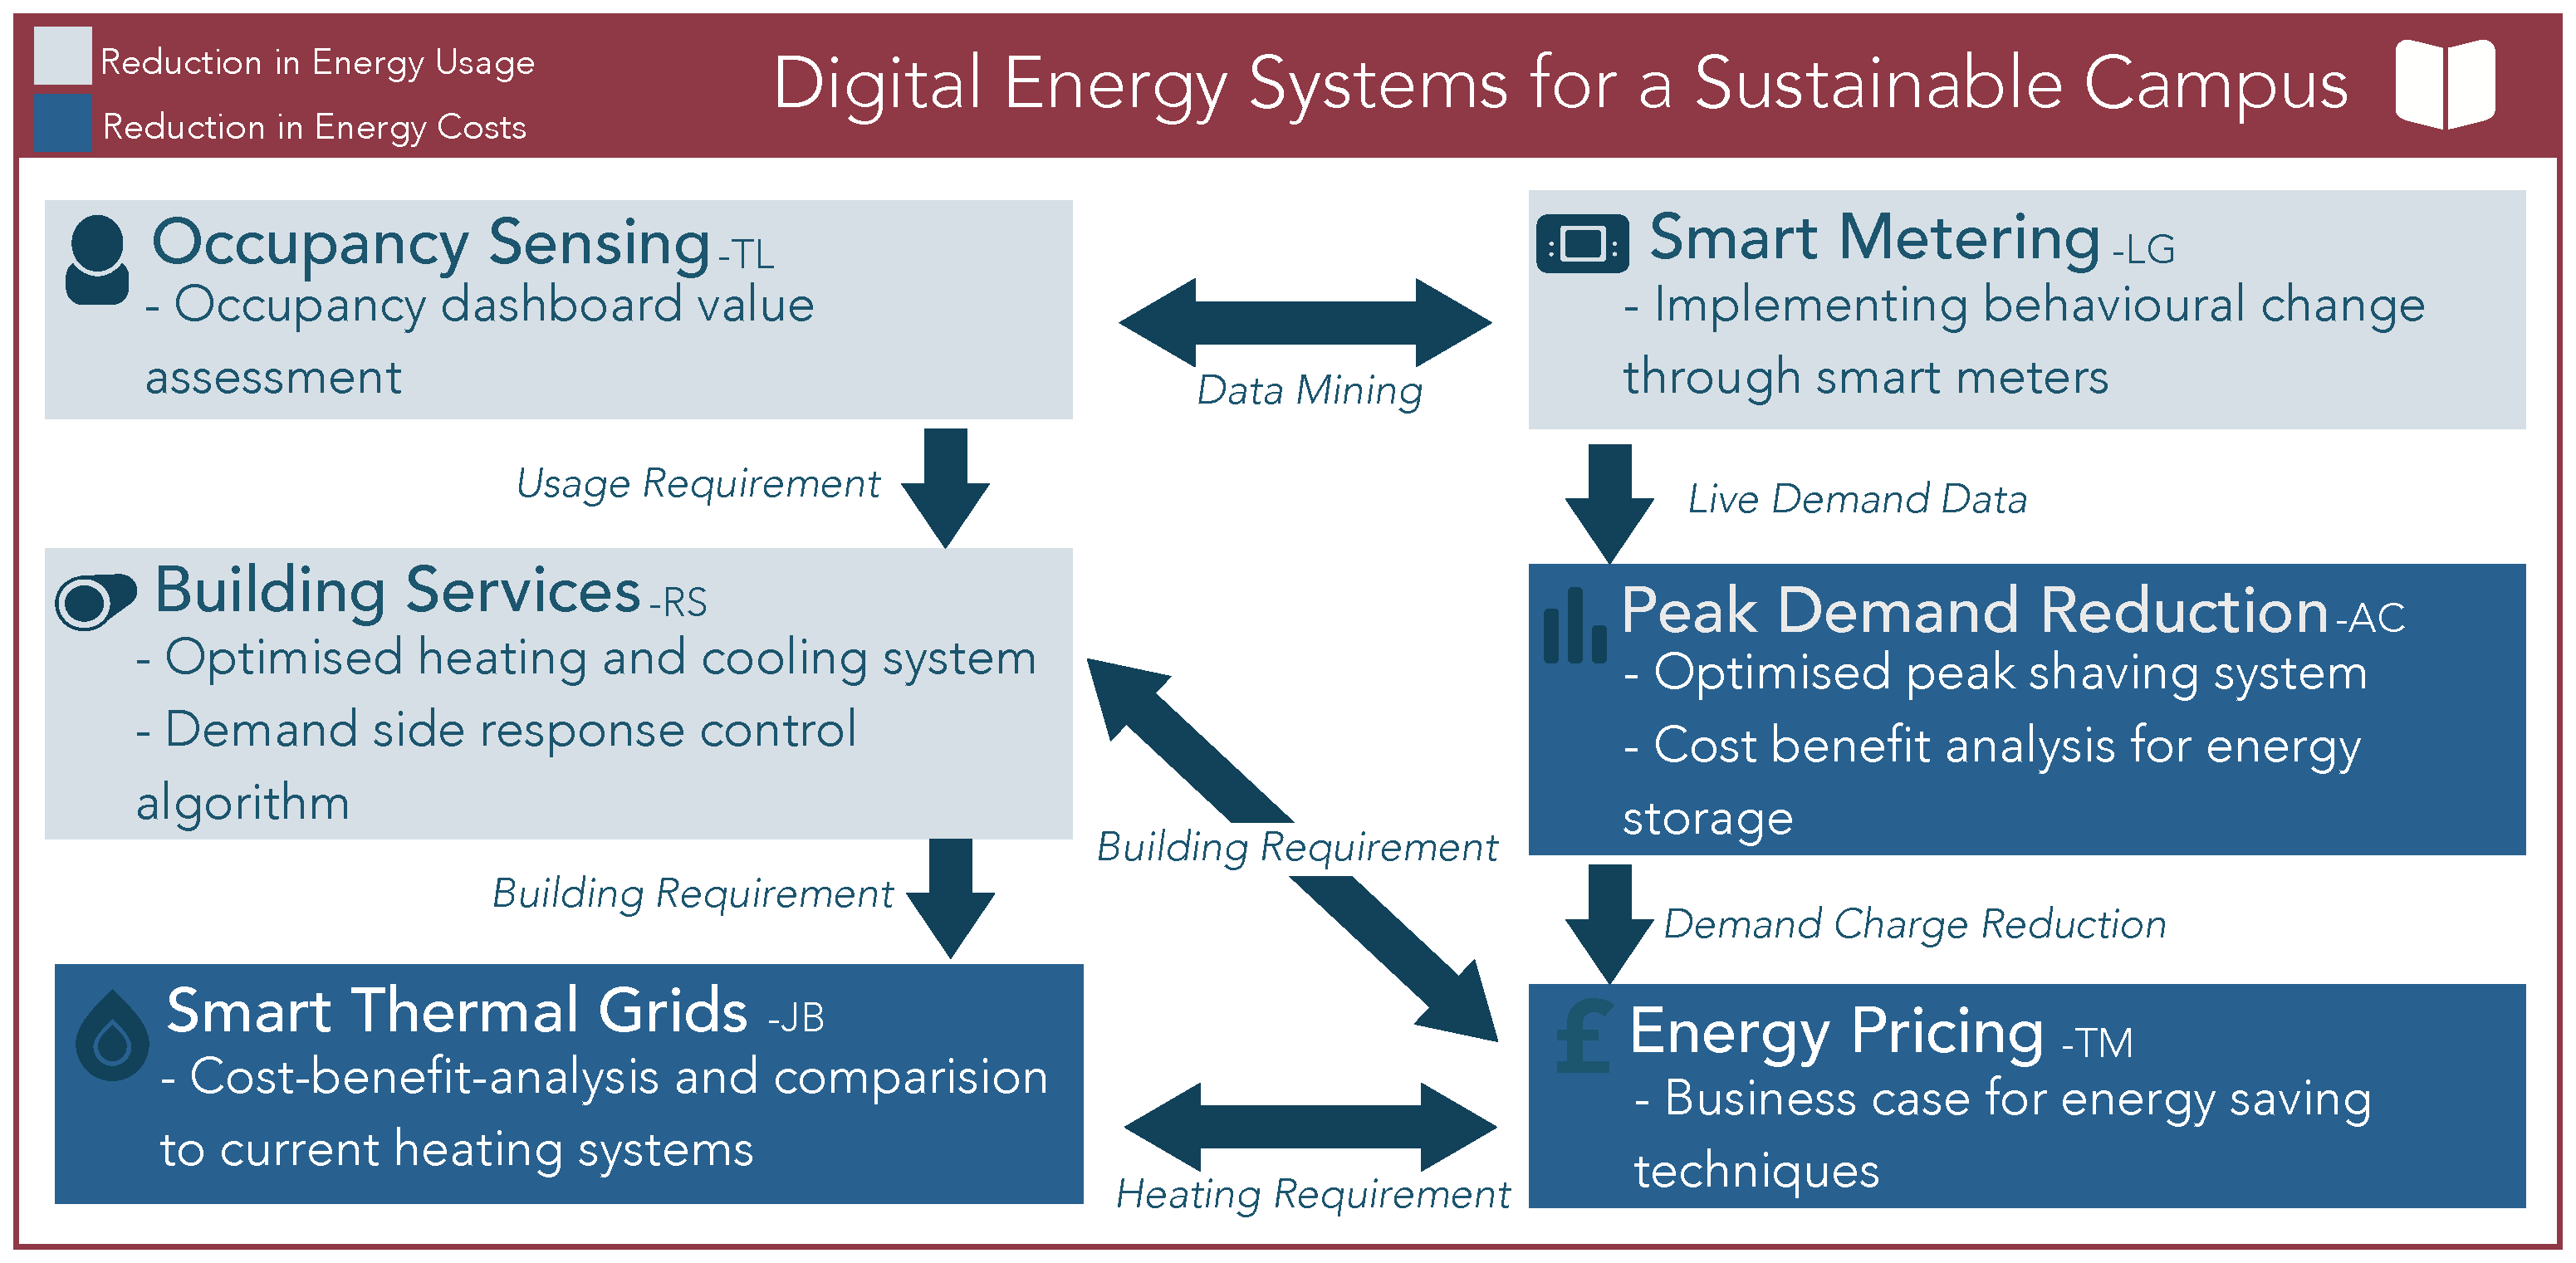
\includegraphics[width=1\textwidth]{diagramGroup.eps}
\caption{Group Design Project Diagram Showing Relationships Between Individual Projects}
\vspace{-20pt}
\label{groupDia}
\end{figure}

Figure \ref{groupDia} shows how the separate subjects of the project are
split, where research in Occupancy Sensing, Smart Metering and Building
Services will evaluate how energy usage in the new campus can be
optimised. Smart Thermal Grid, Energy Pricing and Peak Demand Reduction,
all analyse methods of reducing the University's energy costs. Where new
energy pricing structures coupled with peak demand reduction
technologies, can reduce the load on the grid, helping support
sustainable energies. The 5\textsuperscript{th} year group project will
unite these themes, creating a smart ``brain'' through combining usage
data with new technologies and strategies, providing a business case to
develop sustainable energy services on the new campus, pushing the
University to meet it's carbon neutral 2030 goal
\cite{universi93:online}.

\subsection{Individual Project Aim}\label{individual-project-aim}

The aim of this individual project is to investigate the feasibility of
using an energy storage system (ESS) to reduce charges related to peak
energy demand for the University of Bristol, implemented in the new
Temple Quarter campus. Within the project, the University's peak demand
charges will be analysed and simulated, modelling the bespoke energy
requirements of the campus. Different peak-shaving system architectures
will then be modelled against this usage and charge data, finding an
optimum solution for the system's design concerning the system's capital
cost against savings made from energy bills. This model will provide a
comparison between using a decentralised system, for room by room use,
or a centralised system, being applied to the whole building. The
outputs of the project for 5\textsuperscript{th} year will be a flexible
model which produces an optimum peak-shaving system architecture for a
given University scenario, providing a cost benefit analysis of using
energy storage.

\subsection{Objectives}\label{objectives}

\textbf{Literature Review}

\begin{enumerate}
\item Perform a detailed literature review, and market analysis of energy storage systems used to reduce peak energy demands, highlighting relevant modelling techniques and limitations.
\item Investigate different energy storage solutions, looking at their applicability to a University peak-shaving system, comparing parameters such as; power-ratings, discharge times, charge times and costs.
\end{enumerate}

\textbf{Definition of System Architectures}

\begin{enumerate}[resume]
\item Define peak-shaving system architectures, establishing the key performance variables. This objective will include an investigation of peak demand sensing, smart metering usage, energy storage health monitoring, energy conversion, methods to split supply between an energy storage system and the mains and a comparison between decentralised and centralised energy storage models.

\end{enumerate}

\textbf{Modelling and Analysis}

\begin{enumerate}[resume]
\item Analyse the University’s current peak demand charges; understanding the University’s current demand charge structure and collecting typical energy usage data. Parameters such as time of day and sources of energy peaks will be incorporated.
\item Produce a simulation to optimise the peak-shaving system, comparing metrics including; unit cost and reduction in peak kWh charges based on University billing structure. This model will provide a comparative analysis of the different system architectures. The model will detail savings against the University’s current peak demand charges, being comprised of three stages:
\begin{enumerate}
\item A simulation of the University's a normal energy use case and peak demand charges, for use as a datum.
\item Inclusion of energy storage systems, simulating logic and detailing any prediction methods.
\item An assessment of the use of peak load shedding, supply levelling and forecasting to improve the performance of the model.
\end{enumerate}
\end{enumerate}

\textbf{Evaluation}

\begin{enumerate}[resume]
\item Evaluate results of the simulation, concluding on the effectiveness of different peak-shaving system architectures against particular scenarios. A cost-based analysis will be used to measure the feasibility of the different energy storage systems for the University.
\end{enumerate}

\newpage

\section{Background and Summary of Key Work and
References}\label{background-and-summary-of-key-work-and-references}

The following literature review provides a comprehensive overview of
current research towards using Energy Storage Systems (ESS) to reduce
peaks in energy demand and lower utility costs for the consumer. Peak
demand reduction is synonymous with peak shaving; the ability to control
energy usage from a supplier during intervals of high demand, to limit
or reduce demand charges \cite{schneiderRECPS}, \cite{baldorPS}. As this
project is investigating reducing the peak demand charge for the
University of Bristol, section \ref{peak-demand-charges}, provides an
overview of the University's energy bill, detailing which charges are
effected by peak demand. Section
\ref{current-peak-demand-management-methods-and-energy-storage-systems-usage}
evaluates traditional methods of peak shaving, covering a brief look at
ESSs current usage. Section \ref{peak-shaving-systems-literature-review}
includes a broad range of research of ESSs in different case studies,
optimising the system architecture and analysis on ESSs financial return
on investment (ROI). This research will help in define system
architectures for modelling. Finally section
\ref{peak-shaving-technologies---electrical-storage-system-ess} analyses
the applicability of different ESSs, down-selecting to leave a shortlist
of ESSs to be modelled.

\subsection{Peak Demand Charges}\label{peak-demand-charges}

The University of Bristol's infrastructure, spans across three sites;
the City Centre, Stoke Bishop and Langford. Across these locations, the
majority of facilities receive separate energy bills, allowing a high
degree of granularity in the understanding energy charges
\cite{Jbrentmeet}. The University receives charges bundled together
under four distinct themes \cite{Jbrentmeet}, these have been ranked
below based on the effect a peak-shaving system could have on the
charge.

\begin{enumerate}
\item \textbf{Distribution Use of System (DUoS)} - This bill includes the capacity charge; where the customer pays for a maximum demand level in kW \cite{Deconstr52:online}. The capacity charge is set higher than the actual maximum demand, reducing the risk of breaching this threshold. If breached, the customer incurs substantial penalties, and the supplier increases the threshold for the next billing period. By levelling off peaks in energy demand, the capacity charge threshold can decrease. The capacity charge will be the key focus for the proposed peak-shaving system.
\item \textbf{Transmission Network Use of System (TNUoS)} - These come from three half-hour periods when the UK's National Grid demand is greatest, referred to as Triads. These dates lie between November and February and must be separated by at least ten days during the financial year \cite{TriadsWh7:online}. The average max peak demand across the three Triads \cite{TNUoSTra99:online}, is multiplied by a tariff for the respective zone in cost per kW \cite{TNUoScha93:online}. Combined they become the TNUoS charge, added to the customer's end of year bill. The University has become quite good at forecasting these periods \cite{Jbrentmeet}, making it possible to schedule ESSs to reduce peaks during these periods.
\item \textbf{Unit Charge} - Unit charges come at three different rates, green, amber and red \footcite[See page 27 of][]{SWEB201492:online}, depending on the time of day. Energy costs during red periods are significantly higher (between 5pm-7pm). For Western Power (University's current supplier), there is a 17000\% increase in price during these periods \footcite[25.405 p/kWh in red periods against 0.147p/kWh in green periods][]{SWEB201492:online}. The unit charge will decrease as a consequence of reducing peak demand, where an ESS should only charge in green periods.
\item \textbf{Feed-In Tariff (FIT)} - Based on feeding back energy to the grid. Peak-shaving will not be applicable.
\end{enumerate}

\subsection{Current Peak Demand Management Methods and Energy Storage
Systems
Usage}\label{current-peak-demand-management-methods-and-energy-storage-systems-usage}

Traditionally there are two methods for reducing peak demand for
industrial complexes \cite{schneiderRECPS}. These are:

\begin{itemize}
\tightlist
\item
  \textbf{Load Shedding}: This is reducing energy usage, by switching
  off certain systems during periods of peak demand \cite{6199851}. An
  intelligent scheduling system or a simple forecasting tool can be used
  to execute load shedding \cite{Reducing37:online}, where systems can
  be switched off autonomously or manually. Often load shedding is
  calculated daily using a schedule to set a fixed maximum energy limit
  \cite{6938948}.

  \begin{itemize}
  \tightlist
  \item
    \emph{Limitations}: Forecasting errors can significantly reduce the
    effectiveness of this system, where reactive methods are often
    better \cite{6938948}. Due to the free flow of staff and students at
    the University's facilities, predicting peak demands accurately can
    become a greater challenge.
  \end{itemize}
\item
  \textbf{On-site Generation}: Adding off-the-grid capacity to the
  consumer \cite{schneiderRECPS}. The University currently uses some
  generators to reduce red zone unit charges, supported by
  \cite{shen2016} showing that fuel costs of running a diesel generators
  are lower than energy purchased in red zone rates. If a good return on
  investment is found from purchasing the asset, a diesel generator may
  be feasible to be used alongside an ESS during these periods.

  \begin{itemize}
  \tightlist
  \item
    \emph{Limitations}: The University currently has 0.5MW of
    PhotoVoltaic (PV) installed using nearly all available space
    \cite{Jbrentmeet}. These PV's provide only 0.5\% of the total energy
    demand, meaning the use of on-site generation to offset peak demand
    has a negligible effect in flattening the University's demand if
    used directly.
  \end{itemize}
\end{itemize}

In addition to these limitations, statistics such as ``40\% of energy
use in the campus comes from 5\% of the space, predominantly labs''
\cite{brentemail}, make the University campus a unique case study for
peak demand shaving, where energy storage systems appear more attractive
than traditional techniques.

There are a limited number of peak shaving ESS solutions available
commercially. ABB offers energy-storage, smart-grid products, which
perform load levelling at grid level \cite{abbpeakshave}. These systems
are designed primarily for supply levelling, using forecasting methods
and large ESSs to offset excess energy supply produced from renewable
energies \cite{5559470}, rather than focusing on reducing its customers
energy bills. One Cycle Control have created technologies to regulate
peak-load and mitigate peak demand charges for commercial/industrial
facilities using Li-ion batteries \cite{peakload38:online}. The
technologies proved effective at reducing peak demand charges, but
highlight that the steep cost of the ESSs reduces the system's financial
feasibility \cite{Demonstr51:online}. Being able to sense peak loads and
respond actively will maximise the performance of the system, while the
ESS chosen will have the greatest effect on the systems cost. Section
\ref{peak-shaving-technologies---electrical-storage-system-ess}
evaluates these two different technologies.

\subsection{Peak Shaving Systems Literature
Review}\label{peak-shaving-systems-literature-review}

Acknowledging limitations in commercial peak-shaving ESSs, understanding
current research is crucial to designing efficient system architectures.
Research is grouped, highlighting each section's significance,
identifying areas for further research in work package 2.

\subsubsection{Forecasting and the Use of ESS in Load
Shifting}\label{forecasting-and-the-use-of-ess-in-load-shifting}

Using energy pricing forecasts, an ESS can be switched on to shift
energy costs; purchasing energy at a cheaper rate, using this energy
during peak times. Looking at the gap in energy prices, demand charges
and investment costs for an ESS, NaS, Li-ion and Flow batteries, a basic
on/off algorithm to shift energy purchasing from peak to off-peak times
does not produce a viable return on investment (ROI) \cite{7555795}.
\cite{7555793} highlights that billing peak periods were directly
correlated with peak demand, requiring an even larger ESS to offset this
demand. \cite{5590194} used real hourly spot prices to decide the best
times to turn on and off Vanadium Redox Batteries (VRB) and Polysulfide
Bromide Batteries (PSB). Through sequential quadratic programming (SQP),
battery sizes were optimised, finding PSB's had a better business case
for load shifting. The fundamental differences between \cite{7555795}
and \cite{5590194}, were energy bills targeted and the granularity of
the pricing data used. \cite{6938948} evaluated different control
strategies combining many forecasts to reduce errors in peak shaving
over a monthly period. Weighted and lowest error forecasts were the best
strategies for an energy management system and should be added to the
system architecture if forecasting is used. \cite{Bennett2015122} added
a real-time operator to create an intelligent scheduling system based on
a house to forecast. This system significantly improved the state of
charge of the battery, freeing more energy for use in reducing peaks,
highlighting that forecasts combined with real-time information can
increase the performance of the system further. Work-package 2 will,
therefore, look at using weighted and lowest error forecasts for an ESS,
further understanding the implications of battery health, whilst
work-package 3 will determine if the Universities energy usage data is
responsive enough for a real time intelligent scheduling system.

\subsubsection{Supply Levelling}\label{supply-levelling}

Supply levelling is the most common use for ESS \cite{iearoadmapes},
using large batteries to reduce power fluctuations brought by the use of
renewable technologies \cite{7324861}, \cite{7564619}. Supply levelling
works by storing excess supply, reducing peaks in the grid rather than
in demand. The technology is, therefore, similar to peak shaving.
\cite{Allik20161116} looked at improving supply for a residential home.
Shiftable water heating was identified to account for 50\% of household
electricity use, being modelled as the primary storage device. Excess
load from wind turbines was used to heat water in excess supply periods
bypassing an inverter significantly improving energy losses. This
research is supported by \cite{Leadbetter2012685}. Minimising conversion
through inverters makes a large difference in the efficiency of the
system. An investigation into energy conversion and, using heat as a
secondary storage method will be performed in work-package 2.

\subsubsection{Battery Sizing and Financial
Modelling}\label{battery-sizing-and-financial-modelling}

Numerous studies, analysing the business cases for ESSs have been
conducted. \cite{7555795} and \cite{7555793} model the use ESSs broadly,
to reduce the cost of all energy charges, revealing that the ROI is
unlikely to be feasible beyond 2020. Papers including \cite{1300158} and
\cite{6175723} evaluated financial models for particular case studies,
showing that bespoke solutions achieved greater peak shaving reductions
than returns promised by current generic products \cite{abbpeakshave}.
\cite{7555795}, \cite{7555793}, \cite{1300158}, \cite{6175723} and
\cite{20164002874437} all present a strong arguments that a bespoke
solution for the University will provide a better business case for ESS
than generic commercial technology.

Investigating the benefits of a decentralised system, reducing peaks on
a small scale rather than using one large central ESS, \cite{6604477}
analysed both peak shaving and battery longevity for a large data
centre. Through both experimentation and modelling, \cite{6604477}
showed that when regarding the batteries lifespan, the ability to
regulate load through a series of batteries can be more favourable than
a centralised system. Research conducted by \cite{6348200} and
\cite{Demonstr51:online} also both support using a decentralised system.
A simulation of the impact of lithium-ion batteries operated under a
peak-shaving control algorithm identified cost-optimal battery
configurations and their impact on grid demand, revealing that small
short duration batteries were more favourable and cost effective for the
customer, further supported by \cite{20164002874437}. The model for this
project will assess if this is also the case for a University facility
understanding that a few rooms such as labs contribute to the majority
of peak loads.

\cite{20160601898032}, \cite{Levron201280} all \cite{5371839} all show
alternate ways of optimising the battery sizing configurations.
\cite{5371839}, used a non-numeric modelling method, focusing on
ultra-capacitors to find the optimal ESS. The results emphasised the
constraint of storage capacity, showing an exponential decrease in value
gained after a particular size of ESS. Finding this size for different
University scenarios will be the primary focus of this project's model.
\cite{Levron201280} created an analytical model, using energy bands to
regulate peak load, giving an optimum storage size for a given system;
this was a straightforward and efficient method of modelling battery
usage. \cite{20160601898032} looked specifically at Vanadium Redox Flow
Batteries (VRFB) arguing it benefits over other ESS methods, producing a
MATLAB/Simulink for a residential use case, showing that VRFB can
regulate its frequency efficiently, due to its fast response time, while
still performing peak-shaving services. This project proposes using a
similar modelling technique to \cite{20160601898032}, incorporating more
ESSs.

\subsection{Peak Shaving Technologies - Electrical Storage System
(ESS)}\label{peak-shaving-technologies---electrical-storage-system-ess}

The selected Electrical Storage System (ESS) will govern the cost and
feasibility of a peak shaving system. An ESS converts electrical energy
into a form stored for later use \cite{Chen2009291}. Electrochemical
batteries characterise low maintenance, high round-trip efficiency, long
cycle lives and high energy density's; arguably being the most
appropriate technology for peak shaving \cite{liao2016a},
\cite{Dunn928}. Batteries, therefore, have been chosen as the main focus
for this study. The various storage methods can be characterised for
different uses summaries below:

\begin{itemize}
\tightlist
\item
  \textbf{Energy Management:} for large scale storage, typically used by
  power plants for load levelling and ramping/load following.

  \begin{itemize}
  \tightlist
  \item
    Pumped Hydroelectric Storage (PHS), Compressed Air Energy Storage
    (CAES) and Cryogenic Energy Storage (CES) are the conventional
    technologies for high generation above 100MW. All these methods are
    on a scale too large to be considered for this project.
  \item
    Large-scale batteries, flow batteries, fuel cells, solar fuels, CES
    and Thermal Energy Storage (TES) are suitable for medium-scale
    energy management with capacities of 10 -- 100 MW. These are
    appropriate for consideration for this project.
  \end{itemize}
\item
  \textbf{Power quality:} fast response times improve power quality
  allowing techniques such as the instantaneous voltage drop, flicker
  mitigation and short duration uninterrupted power supply

  \begin{itemize}
  \tightlist
  \item
    Flywheels, Batteries, Superconducting Magnetic Energy Storages
    (SMES), capacitors and ultra-capacitors have millisecond response
    time lower for storage sizes less than 1 MW - suitable perhaps in
    addition to large scale battery. Flywheel efficiency is too low for
    operational use, so has been removed from this study.
  \end{itemize}
\item
  \textbf{Bridging power:} Relatively fast response (\textless{} 1 s)
  but also have relatively long discharge time (hours). The typical
  power rating for these types of applications is about 100 kW -- 10 MW.

  \begin{itemize}
  \tightlist
  \item
    Batteries, flow batteries \cite{flowbatstan}, fuel cells and
    Metal-Air Cells\cite{Chen2009291}, \cite{batuni}.
  \end{itemize}
\end{itemize}

By removing energy storage methods that would not be appropriate for the
system a table was created
\footnote{See table \ref{battabs}, in the Appendices} comparing ESSs.
Batteries along with capacitors provide the response time
\cite{Choudar201521} and efficiencies required to make the system
justifiable, where only rechargeable batteries were compared. From
section \ref{battery-sizing-and-financial-modelling} a model of a
University peak demand reduction system will need to compare different
battery parameters along with their cost, to optimise the model.

\subsection{Previous Bristol University Work
IODICUS}\label{previous-bristol-university-work-iodicus}

\subsection{Battery Capacity
Modelling}\label{battery-capacity-modelling}

\subsection{Battery Selection - Tesla Power-pack
2}\label{battery-selection---tesla-power-pack-2}

Selected Tesla due to lots of readily available information on pricing
and sizes \textbf{Other Competitors} * Eos * BYD

\hl{Very limited information on their costs, technology still maturing (Eos) Can assume that competition will continue to drive the price down, unsure about UK distribution}

\newpage

\section{Battery Storage Technology Key Advantages and
Challenges}\label{battery-storage-technology-key-advantages-and-challenges}

This section discusses and defines how the model was created and the
process used to generate results.

It is important to understand how a battery system can best be utilised
to maximise it's effect. The following section will highlight the
advantages and barriers of using a battery system. Understanding the
advantages will highlight the best way to design a system architectures
which leverages these points. It is this report objective to create
strong arguments to how the system will overcome barriers to entry,
laying out how all the assumptions in the model overcome these issues
and address any qualitative issues in the following section

\textbf{Advantages}

\begin{itemize}
\tightlist
\item
  Reducing Electricity Bills:

  \begin{itemize}
  \tightlist
  \item
    Reducing the DUoS Charges
  \item
    Reducing Triad Charges
  \item
    Playing on the frequency response market (beyond project scope)
  \item
    Reducing capacity charges
  \end{itemize}
\item
  Supply Levelling:

  \begin{itemize}
  \tightlist
  \item
    Leveraging maximum use of PV's and other renewable energy sources
  \item
    Providing a fully predictable energy profile for new building.
    Useful in negotiating price when new power capacity has to be
    installed ( very relevant to the new Bristol campus), saves paying
    for the new connection. \cite{wpMWMD}
  \end{itemize}
\item
  Emergency Power: Providing backup generation in the case of power
  cuts. Can support crucial systems alleviating risks associated with
  loss of power
\item
  Sustainability:

  \begin{itemize}
  \tightlist
  \item
    Reducing peak load, reduces losses on the network. There is a green
    argument for running diesel generators in peak times. Batteries are
    a highly more sustainable.
  \item
    Ensures self consumption of renewables
  \end{itemize}
\end{itemize}

\textbf{Challlenges}

\begin{itemize}
\tightlist
\item
  Costs of Purchase too high:

  \begin{itemize}
  \tightlist
  \item
    Installation Costs too high, too complex -
    \hl{difficulty of retrofitting?}
  \item
    Unit Price of the battery is too high - (kWh)
  \item
    Additional equipment cost, inverters
  \item
    Maintenance cost
  \end{itemize}
\item
  Lifetime/ longevity of the battery too low, replacement costs/
  dismantling cost make battery installation unfeasible

  \begin{itemize}
  \tightlist
  \item
    Unpredictability in cycle life of the battery may mean that lifetime
    is much lower than all good predictions
  \end{itemize}
\item
  Finance not feasible

  \begin{itemize}
  \tightlist
  \item
    Loan Interest \textgreater{} Savings
  \item
    Negative NPV
  \end{itemize}
\item
  Frequent change of regulation may mean that costs shift to reduce
  battery savings, use for reducing DUoS is still favoured by energy
  companies. May change if lots of people take up using batteries in
  this manner.
\item
  Barriers to entry

  \begin{itemize}
  \tightlist
  \item
    Laws/ regulations
  \item
    Penalisation from energy companies
  \end{itemize}
\item
  Negative environmental effects: Uses of large scale quantities may be
  hold undesired environmental risks
\item
  Risk of injury/ explosion. Large batteries that overload, hold a very
  high risk of explosion. Battery system monitoring is key to ensuring
  the battery operates with in it's limits
\item
  Technology still maturing, Li-ion batteries have not been used in this
  manner before, for extended periods of time
\end{itemize}

\subsection{Battery Economics}\label{battery-economics}

The main objective of this project is to create a business case for
using a battery system to reduce energy bills. Ultimately the model aims
to produce the information required to justify whether investing in
batteries is feasible and advise on the best battery to buy based on
it's capacity and it's power rating. Due to the readily available
commercial information of Tesla's Power-pack 2, this battery system was
used to model financial feasibility and optimal product.

There are 3 ways the model will evaluate the value of the battery
system, these are: \emph{pay-back period}, \emph{total-savings} (over a
designated period of time) and \emph{net present value} (calculated for
different discount rates). Each of these methods results will be
compared to crediting the merits and pitfalls of each to understand
which battery system is the optimum for the system.

\textbf{NPV Calculation:} As the battery is a large up front cost, it is
likely that the battery will be purchased on financing this means that
interest on the loan has to be paid each year reducing the battery
value. Additionally the battery will degrade in performance over time,
this is key to understanding the value of the product over its life
time. Using an Initial return rate \hl{Add return rate calc here} the
maximum discount rate can be found for a few batteries (using the
extremes). This can then be used to set different discount rates, where
0 is used to illustrate the payback of the battery. Even with the
battery degrading, it can be predicted that the battery will continue to
degrade until failure.
\hl{The net present value (NPV) is a way to examine costs and revenues while accounting for the time value of money. If the NPV of a system is positive, then the investment is predicted to provide a return on investment greater than the initial and ongoing cash expenditures associated with ownership of the system. A negative NPV indicates the returns are worth less than the cash outflows and the investment does not show a financial benefit, although unquantified benefits may be present.}
\cite{diorio2015economic} Total-savings is the measure of net present
value when the discount rate is 0.

\textbf{Payback Period:}
\hl{The payback period (PBP) is the time in years it takes for project savings to equal or exceed the initial cost of the investment. This metric is included because of its ability to quickly communicate tangible value of a project. A system which yields a very short payback period is typically a profitable one because subsequent years of the project result in pure revenue for the system owner. A system which cannot be paid back over the lifetime of the system is a poor investment because money is still owed when the system is retired and no longer able to generate revenue. The payback period is reported as the first time where the project savings exceeds the debt, but care must be taken to also consider additional cash expenditures in later years.}
\cite{diorio2015economic} The this model looks at the lifetime of
investing in one battery system over a period of time so additional cash
expenditure is ignored in this model.

\subsection{Battery Costing}\label{battery-costing}

\hl{explanation of the Power-pack 2 costs, including warranty, maintenance, installation and any other additional costs. Discussion of the falling costs of lithium battery prices, refer to Diagram}

\begin{figure}[H]
  \centering
  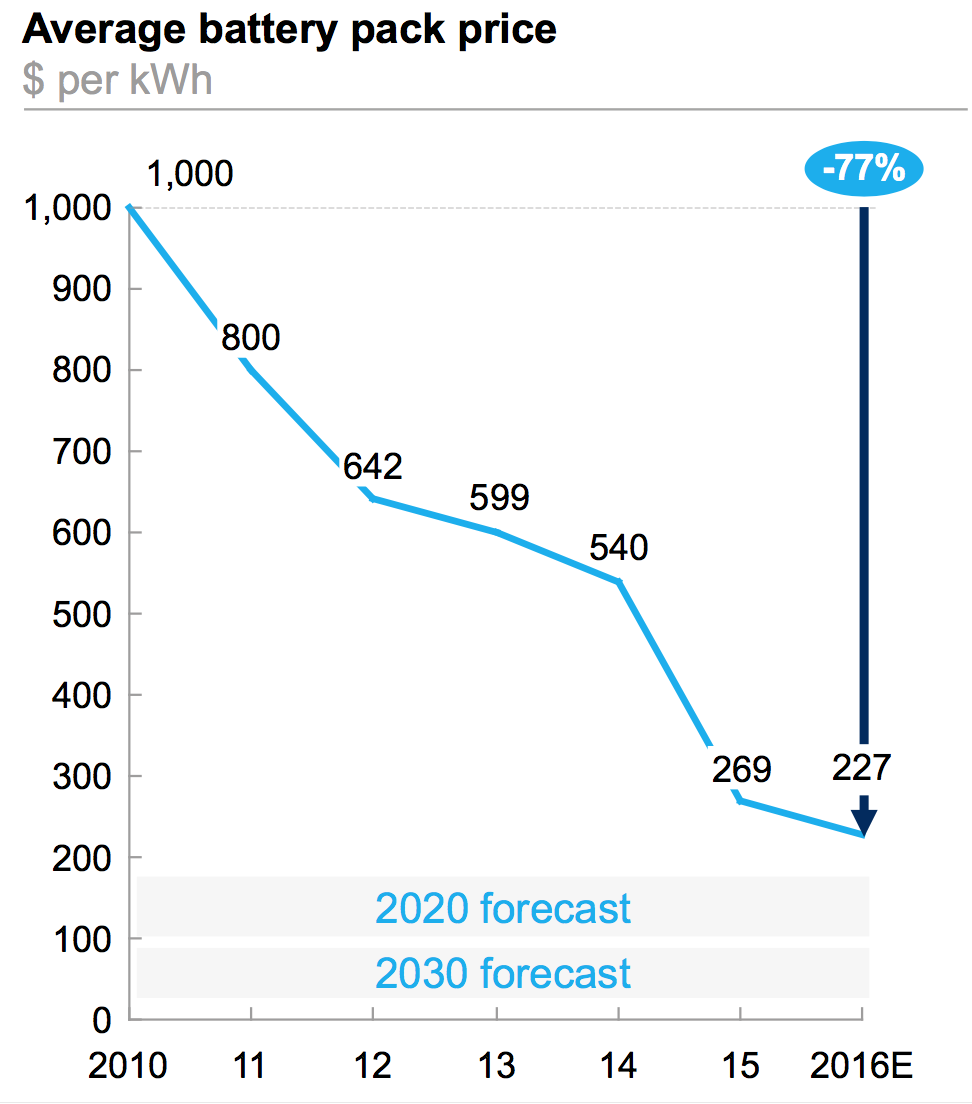
\includegraphics[trim = 0 0 0 0, clip, width=0.5\textwidth]{mckBatPrice.png}
  \caption{Plot of Battery Prices Reduction for 2010-2016 and Predictions for Future battery Prices \cite{mckBat}}
  \label{mckBatPrice}
\end{figure}

\hl{Discussion of Li-ion Battery Falling costs, why now or the 5 year time period of the campus is a good time to buy, installation costs, probably large when retrofitting to an existing building, although the technology comes as almost plug and play, assume will need to be connected to where the mains supply enters the building in order to work in tandem with mains supply Other technology required such as inverters e.c.t.}

\subsection{Battery Lifetime Assessment - Understanding Battery
Degradation}\label{battery-lifetime-assessment---understanding-battery-degradation}

The below figure shows the typical profile a Li-ion battery follows as
it degrades over time:

\begin{figure}[H]
  \centering
  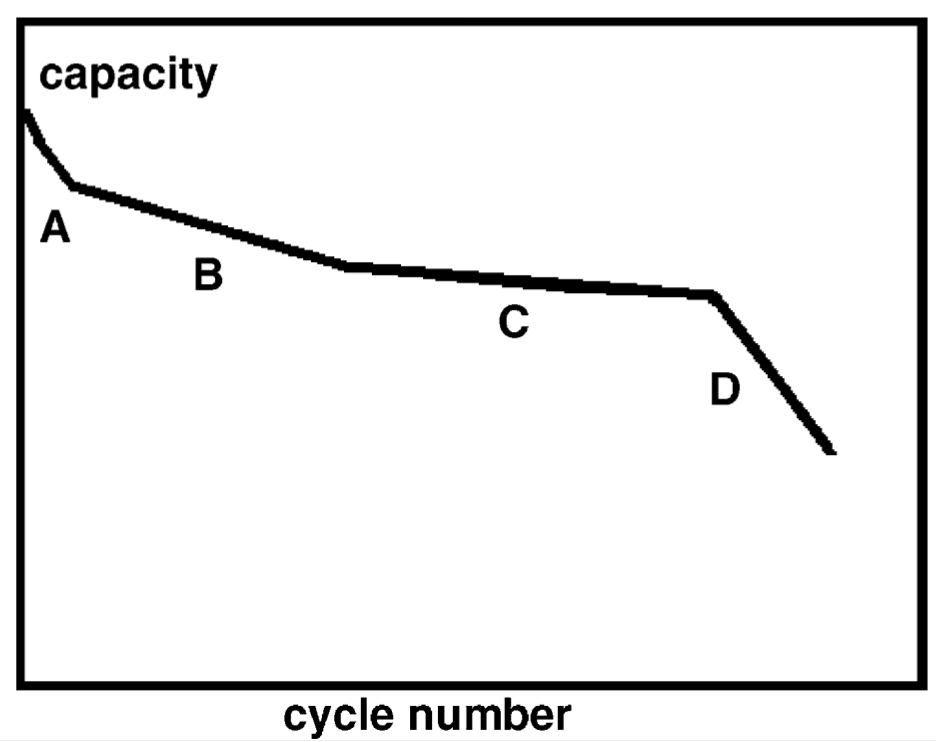
\includegraphics[trim = 0 0 0 0, clip, width=0.35\textwidth]{batCapGen.png}
  \caption{Plot of the General Relationship between battery capacity and cycle number \cite{spotnitz2003simulation} }
  \label{batCapGen}
\end{figure}

After the battery degrades below 80\% of it's new maximum capacity, the
battery is regarded to be at its' end of life phase. It is important to
note that there potential for a large amount of capacity to be delivered
beyond this point, however as seen in figure \ref{batCapGen}, the
battery tends to degrade a lot quicker. There are also issues with power
degradation

The literature review revealed these factors to have the greatest effect
on the rate in which the battery decays:

\begin{itemize}
\item
  Temperature: By running the battery at a temperature too hot or two
  cold, the battery will degrade much quicker
  \hl{Include numerical prediction here with reference}
  \cite{rong2006analytical}
\item
  Charging:

  \begin{itemize}
  \tightlist
  \item
    Charging Level: The cycle life of a battery can be increased by
    reducing the cut off voltage of the battery.
    \hl{Battery voltage will be fixed at either high voltage three phase or at single phase 240V, instead current drawn by the battery will very.}
    Decreasing the current drawn therefore will extend the battery cycle
    life, give the battery a partial charge instead of fully charing it.
    This has a similar effect to working at a lower DoD.
    \cite{Choi2002130}

    \begin{figure}[H]
    \centering
    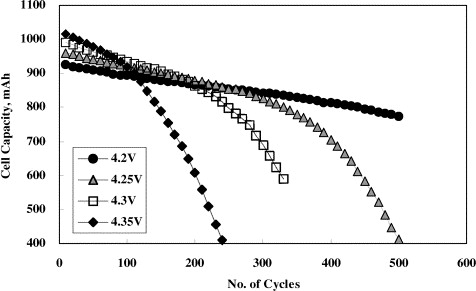
\includegraphics[trim = 0 0 0 0, clip, width=0.5\textwidth]{capVol.jpeg}
    \caption{Plot of the Relationship Between Battery Cycle Life and Voltage of Charge \cite{Choi2002130} }
    \label{capVol}
    \end{figure}
  \item
    Overcharging: By charging the battery too its' full capacity the
    battery or continuing to charge the battery beyond its designed
    voltage, the battery capacity can quickly degrade.
    \hl{The battery becomes unstable if inadvertently charged to a higher than specified voltage. Prolonged charging above 4.30V on a Li-ion designed for 4.20V/cell will plate metallic lithium on the anode. The cathode material becomes an oxidising agent, loses stability and produces carbon dioxide (CO2). The cell pressure rises and if the charge is allowed to continue, these can cause the temperature inside the cell to increase, furthering the reduction in the batteries capacity. A fully charged battery has a lower thermal runaway temperature and will vent sooner than one that is partially charged. All lithium-based batteries are safer at a lower charge.}
    \cite{Charging53:online} Due to these two issues the battery should
    stop charging once it reaches a threshold below its maximum value.
  \item
    Charging Rate:
    \hl{The capacity reduction at high discharge rates occurs because the transformation of the active chemicals cannot keep pace with the current drawn. The result is incomplete or unwanted chemical reactions and an associated reduction in capacity}
    \cite{BatteryL10:online}
  \end{itemize}
\item
  Useage

  \begin{itemize}
  \tightlist
  \item
    Over Depletion: Leaving the battery fully empty for too long can
    have detrimental effects on capacity. It is common for battery
    management systems (BMS), particularly in consumer electronics to
    power the device off at a threshold above 0, to negate some of
    effects of low energy storage \cite{Prematur82:online}.
    \hl{Add further evidence here}
  \item
    Speed of Depletion: The rate in which the battery is discharge can
    have a strong effect on the battery life time. The images below
    shows the effect on discharge rate on the rated capacity of a
    battery. \cite{BatteryL10:online},\cite{Effectso69:online}

    \begin{figure}[H]
       \centering
       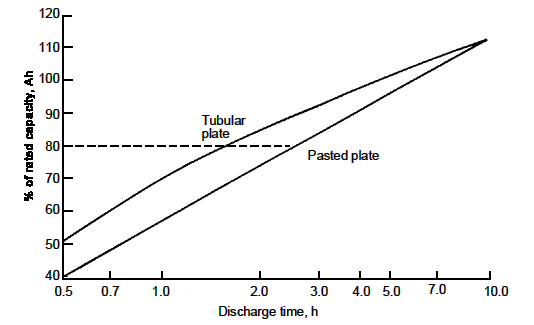
\includegraphics[trim = 0 0 0 0, clip, width=0.5\textwidth]{disRate.png}
       \caption{Plot of the Relationship Between Discharge Time and its' Effect on the Rated Capacity of a Battery \cite{Effectso69:online}}
       \label{disRate}
     \end{figure}
  \end{itemize}
\item
  Depth of Discharge (DoD): Depth of discharge is related to the number
  of \textbf{active} chemicals transformed with each charge/ discharge
  cycle. One full cycle is seen as when the battery is charged to its
  full current capacity (noting that the capacity will degrade over
  time, making each cycle length smaller). It has been cited that there
  is a logarithmic relationship between depth of discharge and the cycle
  life of the battery
  \cite{BatteryL10:online}.\hl{Note the graph above is for Lead-Acid batteries, but also holds true for Li-ion by restricting the possible DOD in the application, the designer can dramatically improve the cycle life of the product. Similarly the user can get a much longer life out of the battery by using cells with a capacity slightly more than required or by topping the battery up before it becomes completely discharged.}
  \cite{BatteryL10:online}

  \begin{figure}[H]
    \centering
    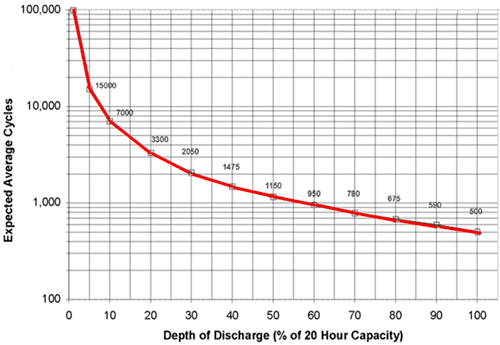
\includegraphics[trim = 0 0 0 0, clip, width=0.5\textwidth]{dodLog.png}
    \caption{Plot of Depth of Discharge vs Cycle Life \cite{BatteryL10:online}}
    \label{dodLog}
  \end{figure}

  \begin{figure}[H]
  \centering
  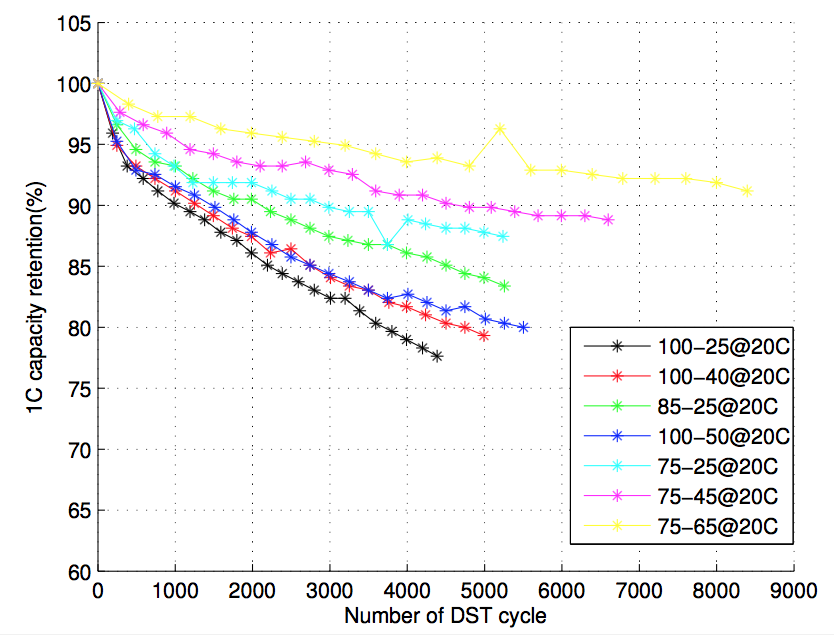
\includegraphics[trim = 0 0 0 0, clip, width=0.5\textwidth]{SoCgraph.png}
  \caption{Plot of the Measured  Relationship between battery State of Charge and it's Effect on the Cycle Number lifetime \cite{xu2016modeling}}
  \label{SoCgraph}
    \end{figure}
\end{itemize}

\newpage

\section{Battery Model Definition}\label{battery-model-definition}

Understanding the key design parameters highlighted in section
\ref{Development-of-Model-Advantages-and-Barriers-Assessment}. The model
was created to capture as many of these drivers to maximise the models
validity. Data was obtained for Senate house (a large University
office/study space building). This data was manipulated to create a
representative energy profile for the Senate and then the New Campus.

\hl{Overview of the final system Diagram}

\subsection{Model Development
Requirements}\label{model-development-requirements}

\subsubsection{0 vs 3D Modelling
Approach}\label{vs-3d-modelling-approach}

\hl{The 0D modelling approach is a technique widely used in the development cycle of a product, typically in the early steps of the cycle. The objective of the 0D model is to define the main characteristics and performance of the products. A 3D model is implemented later in the product development cycle to get a detailed analysis, to verify the accuracy of the 0D model and to predict risks and failures. In a 0D model, the system dynamics is a function of the time while in a 3D model, the system dynamics is a function of the time and the space. A 0D model is much simpler and faster to solve than a 3D model. This enables to run a large number of simulations and explore a large design space for our product.}
\autocite{ZeroDMod80:online} Due to the level of accuracy required to
achieve this reports objectives in the model and the timeframe that the
model had to be constructed in a 0D model was created using the
variables stated in section
\ref{input-parameters-and-multi-battery-simulation}.

\subsubsection{Code Optimisation}\label{code-optimisation}

\hl{A time-based iterative approach, based around a zero dimensional approach, has been selected to model a large variety of different batteries. Running the simulation through time requires calculating large matrices which are number of days $\times$ 1440 (minutes in a day). The model should be optimised for performance to ensure that running times are minimised. This will help to improve model development and reduce data collection time. Possible methods to optimise the performance of MATLAB scripts are:
• Vectorisation – data can be stored and manipulated within multidimensional arrays. Using vector operations, rather than manually moving and manipulating data inside the array, can greatly improve model speed.
• Avoiding heavy processing MATLAB functions such as the linear interpolation function. Instead, simplified versions can be developed to perform the same task.
• Initialising variables within the model. All arrays should be initialised within the memory. This prevents MATLAB from needing to create extra space within the memory each time a value is entered into an array. This is especially important when dealing with large datasets, as it can prevent running out of memory.
• Parallel processing for loops can be used for independent repeating tasks. This can be applied when multiple batteries as each loop is independent of the other.}

\subsubsection{User Interface}\label{user-interface}

\hl{The model developed through this research project is likely to be used in the group project in the following year. Consequently, it is important that the model is easy to run and use. A range of inputs are required for each lagoon which should be easily configured and managed. This will also improve ease of data collection for this project and reduce the risk of introducing a systemic error, associated with the user entering incorrect inputs. Model inputs should therefore be largely removed from the MATLAB script and kept within input files.
A level of intelligence should also be built into the model to determine if the user inputs are valid. This would increase the robustness of the model and prevent errors from occurring within the model. It will also help to improve the stability of the model, as incorrect data will be less likely to be inputted. However, this requirement is likely to be more relevant in the following year, when multiple users are generating data from the energy model. It is important that the model is able to handle a range of variable input conditions}

\subsubsection{Ease of Development}\label{ease-of-development}

\hl{Due to the nature of mathematical modelling, it is essential the model is structured to allow for development and expansion as the project progresses. This allows functionality to be added to the model without a large amount of upfront work. It also improves the speed at which changes can be implemented within the model.
The use of functions within the script allows elements of the code to be re-used across the model. Nested functions (functions defined in the body of a parent function) can also be used when a large number of variables are required to pass back and forth between functions. This also provides modularity within the function and can reduce the amount of repeated code. It is important that a function based approach is taken through the development of the model in this research project due to the expected size and complexity of the model. Without this, the model is likely to have a poor structure and will be much harder to develop and debug.}

\subsection{Creation of Senate House Billing
Model}\label{creation-of-senate-house-billing-model}

Data was received for Senate house, giving usage in kWh for the previous
half hour period. A bill was also provided for a months energy use at
the Victoria rooms (another Bristol University building used for
lecturing, offices and teaching classes). A meeting with John Brenton
\hl{add reference} clarified that billing profiles for both buildings
were identical.

In order to gauge the size and power requirements needed for a building
the size of Senate house, a minute by minute usage profile needed to be
created and then cross checked against a representative bill to
understand how the different charges are broken down and highlight
charges to target the design of the battery system architecture too.

Using the half hourly usage data of senate house for a year, usage plots
were created for different days in the year. It was clear that the was a
major difference between energy demand during the weekend and during the
week, shown in \ref{Development-c4}. Total energy consumption was 3
times greater over the weekdays than the weekend. When creating at usage
data, it was imperative to make sure that weekday's and weekend matched
completely in order to give an accurate representation about the energy
usage.\\

\begin{figure}[H]
 \centering
 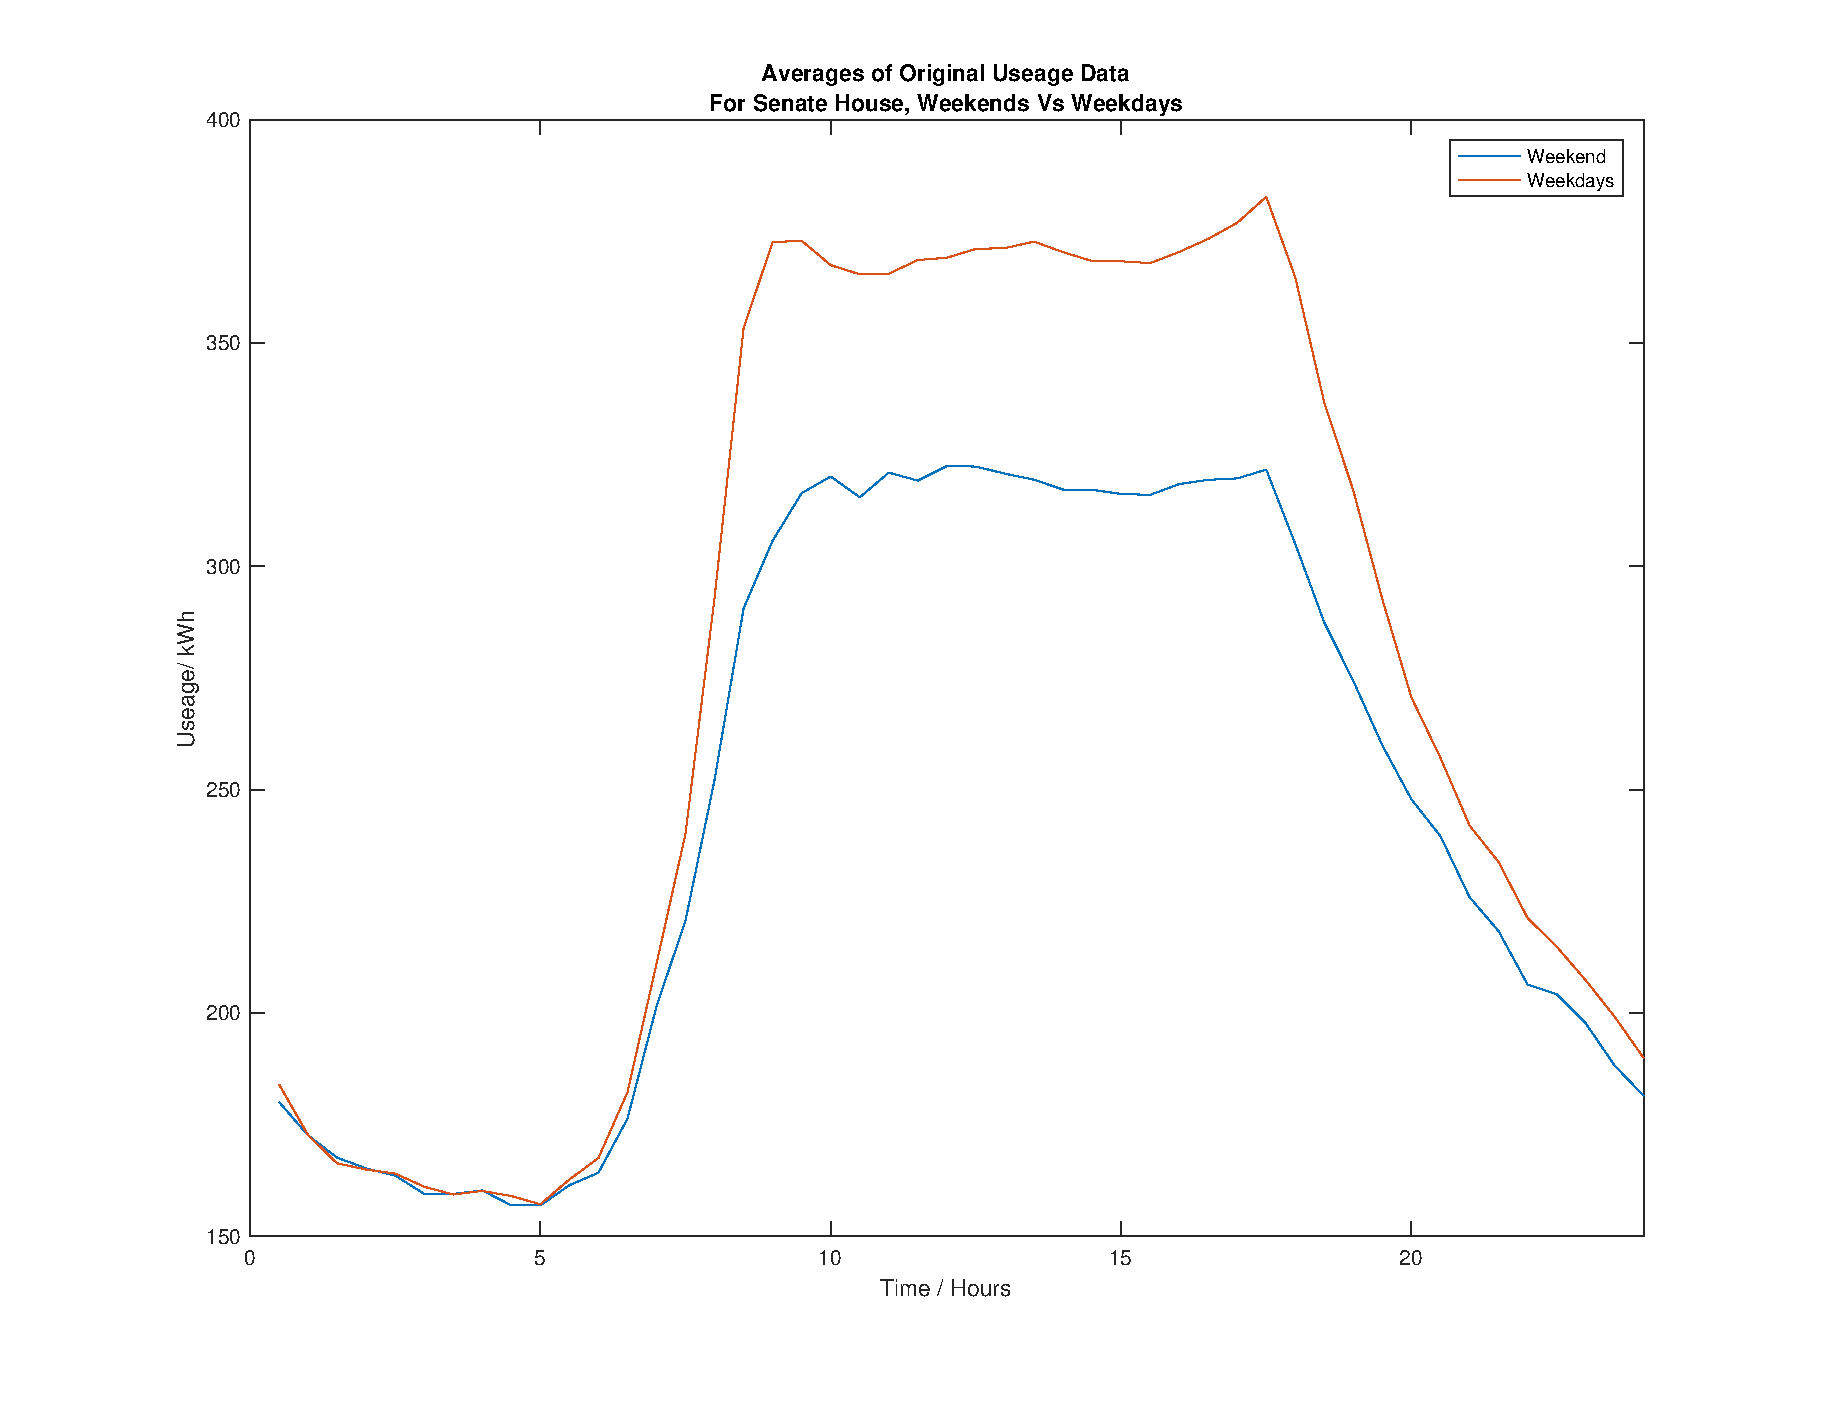
\includegraphics[trim = 50 50 30 50, clip, width=0.5\textwidth]{Development-c4.eps}
 \caption{Plot of Mean Senate House Weekday and Weekend Usage}
 \label{Development-c4}
 \end{figure}

This data was good at giving a rough estimation of the battery size
needed to produce some impact on the Universities energy bills.

\subsubsection{Representative Bill
Creation}\label{representative-bill-creation}

\begin{figure}[H]
 \centering
 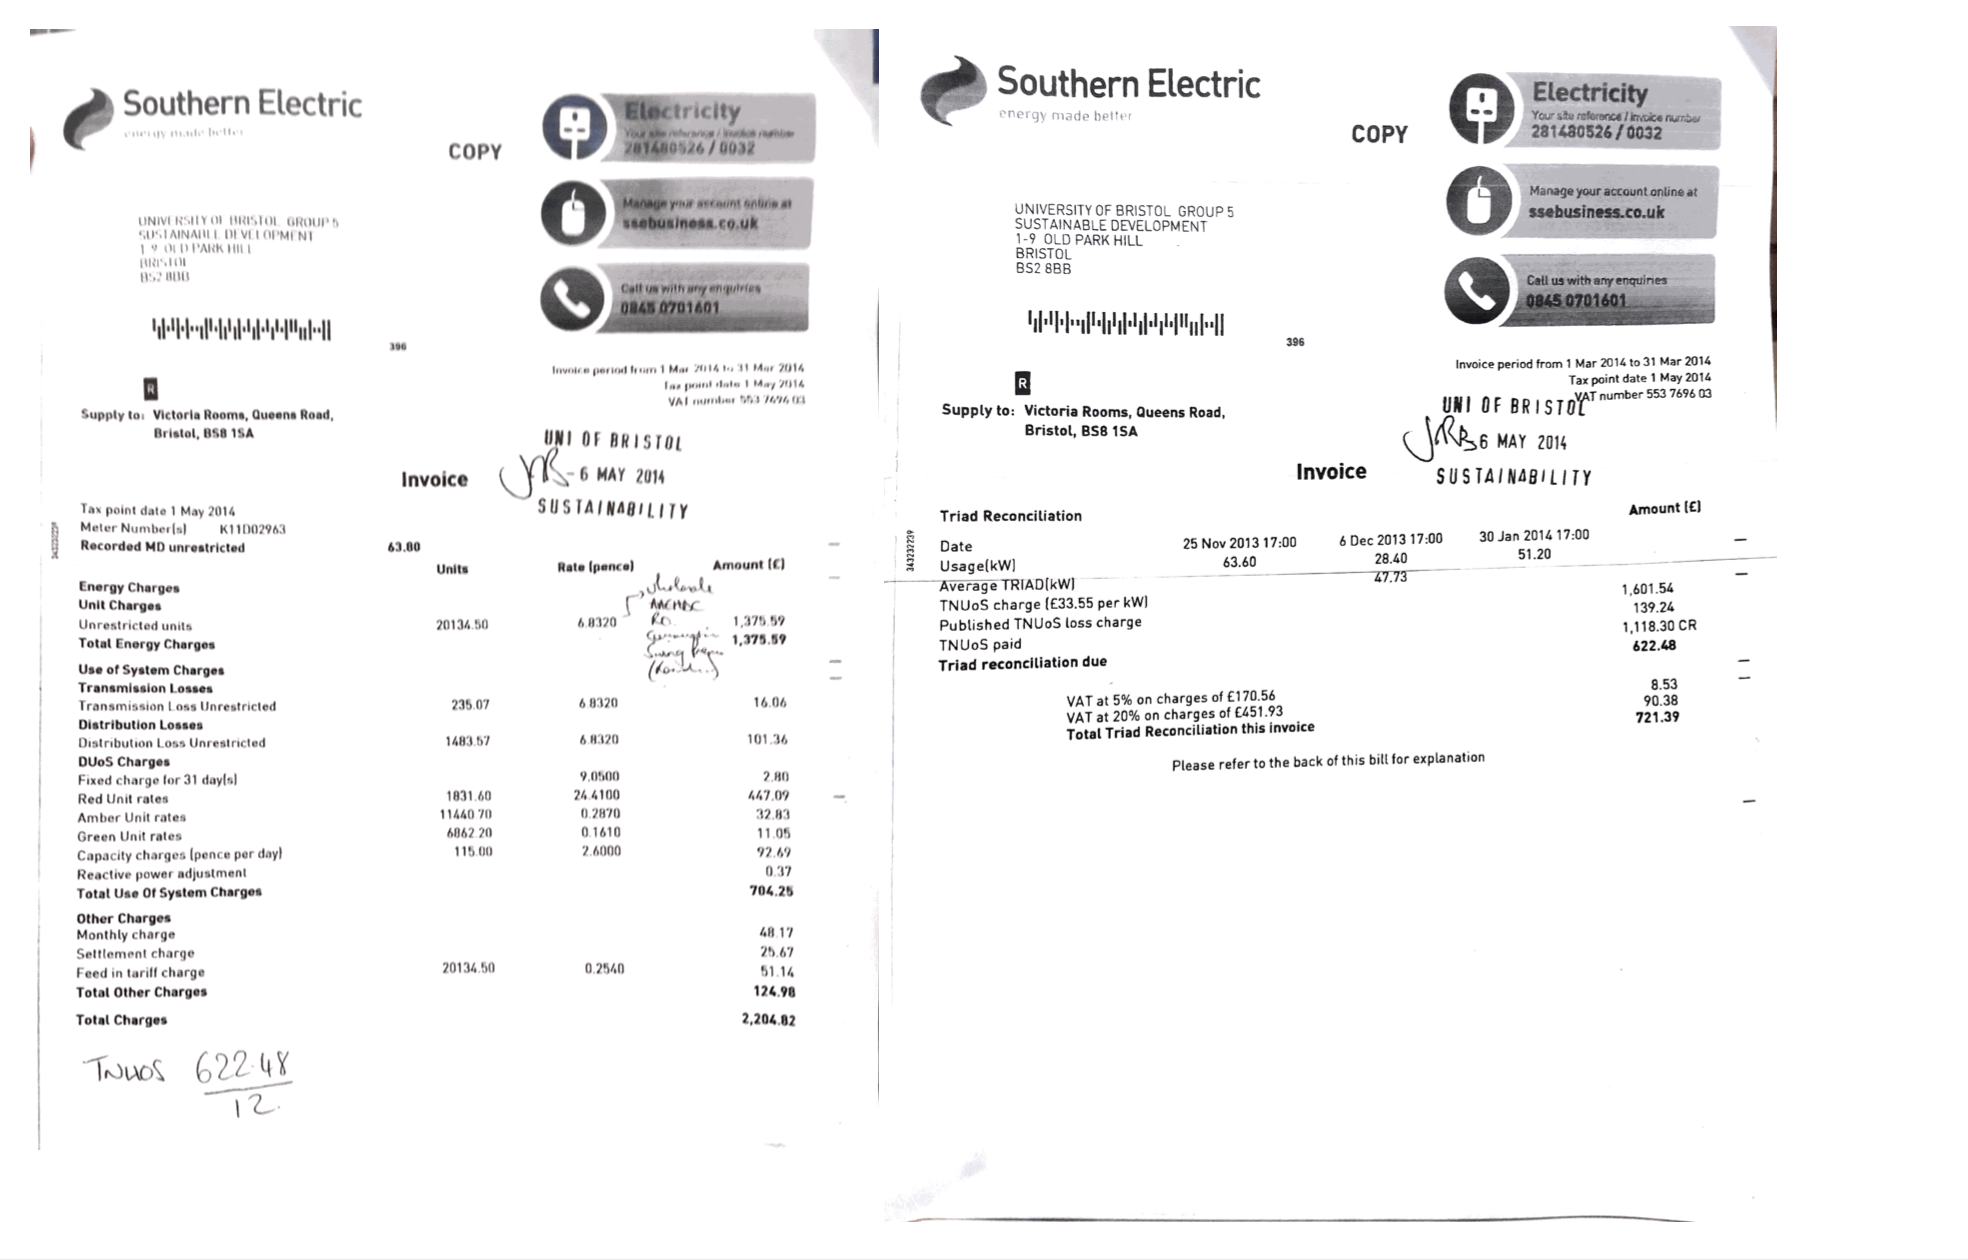
\includegraphics[trim = 0 0 0 0, clip, width=0.5\textwidth]{Development-38.png}
 \caption{Image of Energy Bill For Victoria Rooms}
 \label{Development-38}
 \end{figure}

Figure \ref{Development-38} shows a typical electricity bill for a
University building. It is clear the red unit rates make up the largest
part of the DUoS Charge and roughly 20\% of that months total recorded
charges. Instead capacity charges made up only 4\% of the total bill.
This realisation meant that the focus of the model would be to start by
reducing the red rate charge through load shifting, and explore other
charges if this proved to not be effective to offset investment costs.
Figure \ref{Development-50} highlights the significance of the different
unit costs.

\begin{figure}[H]
 \centering
 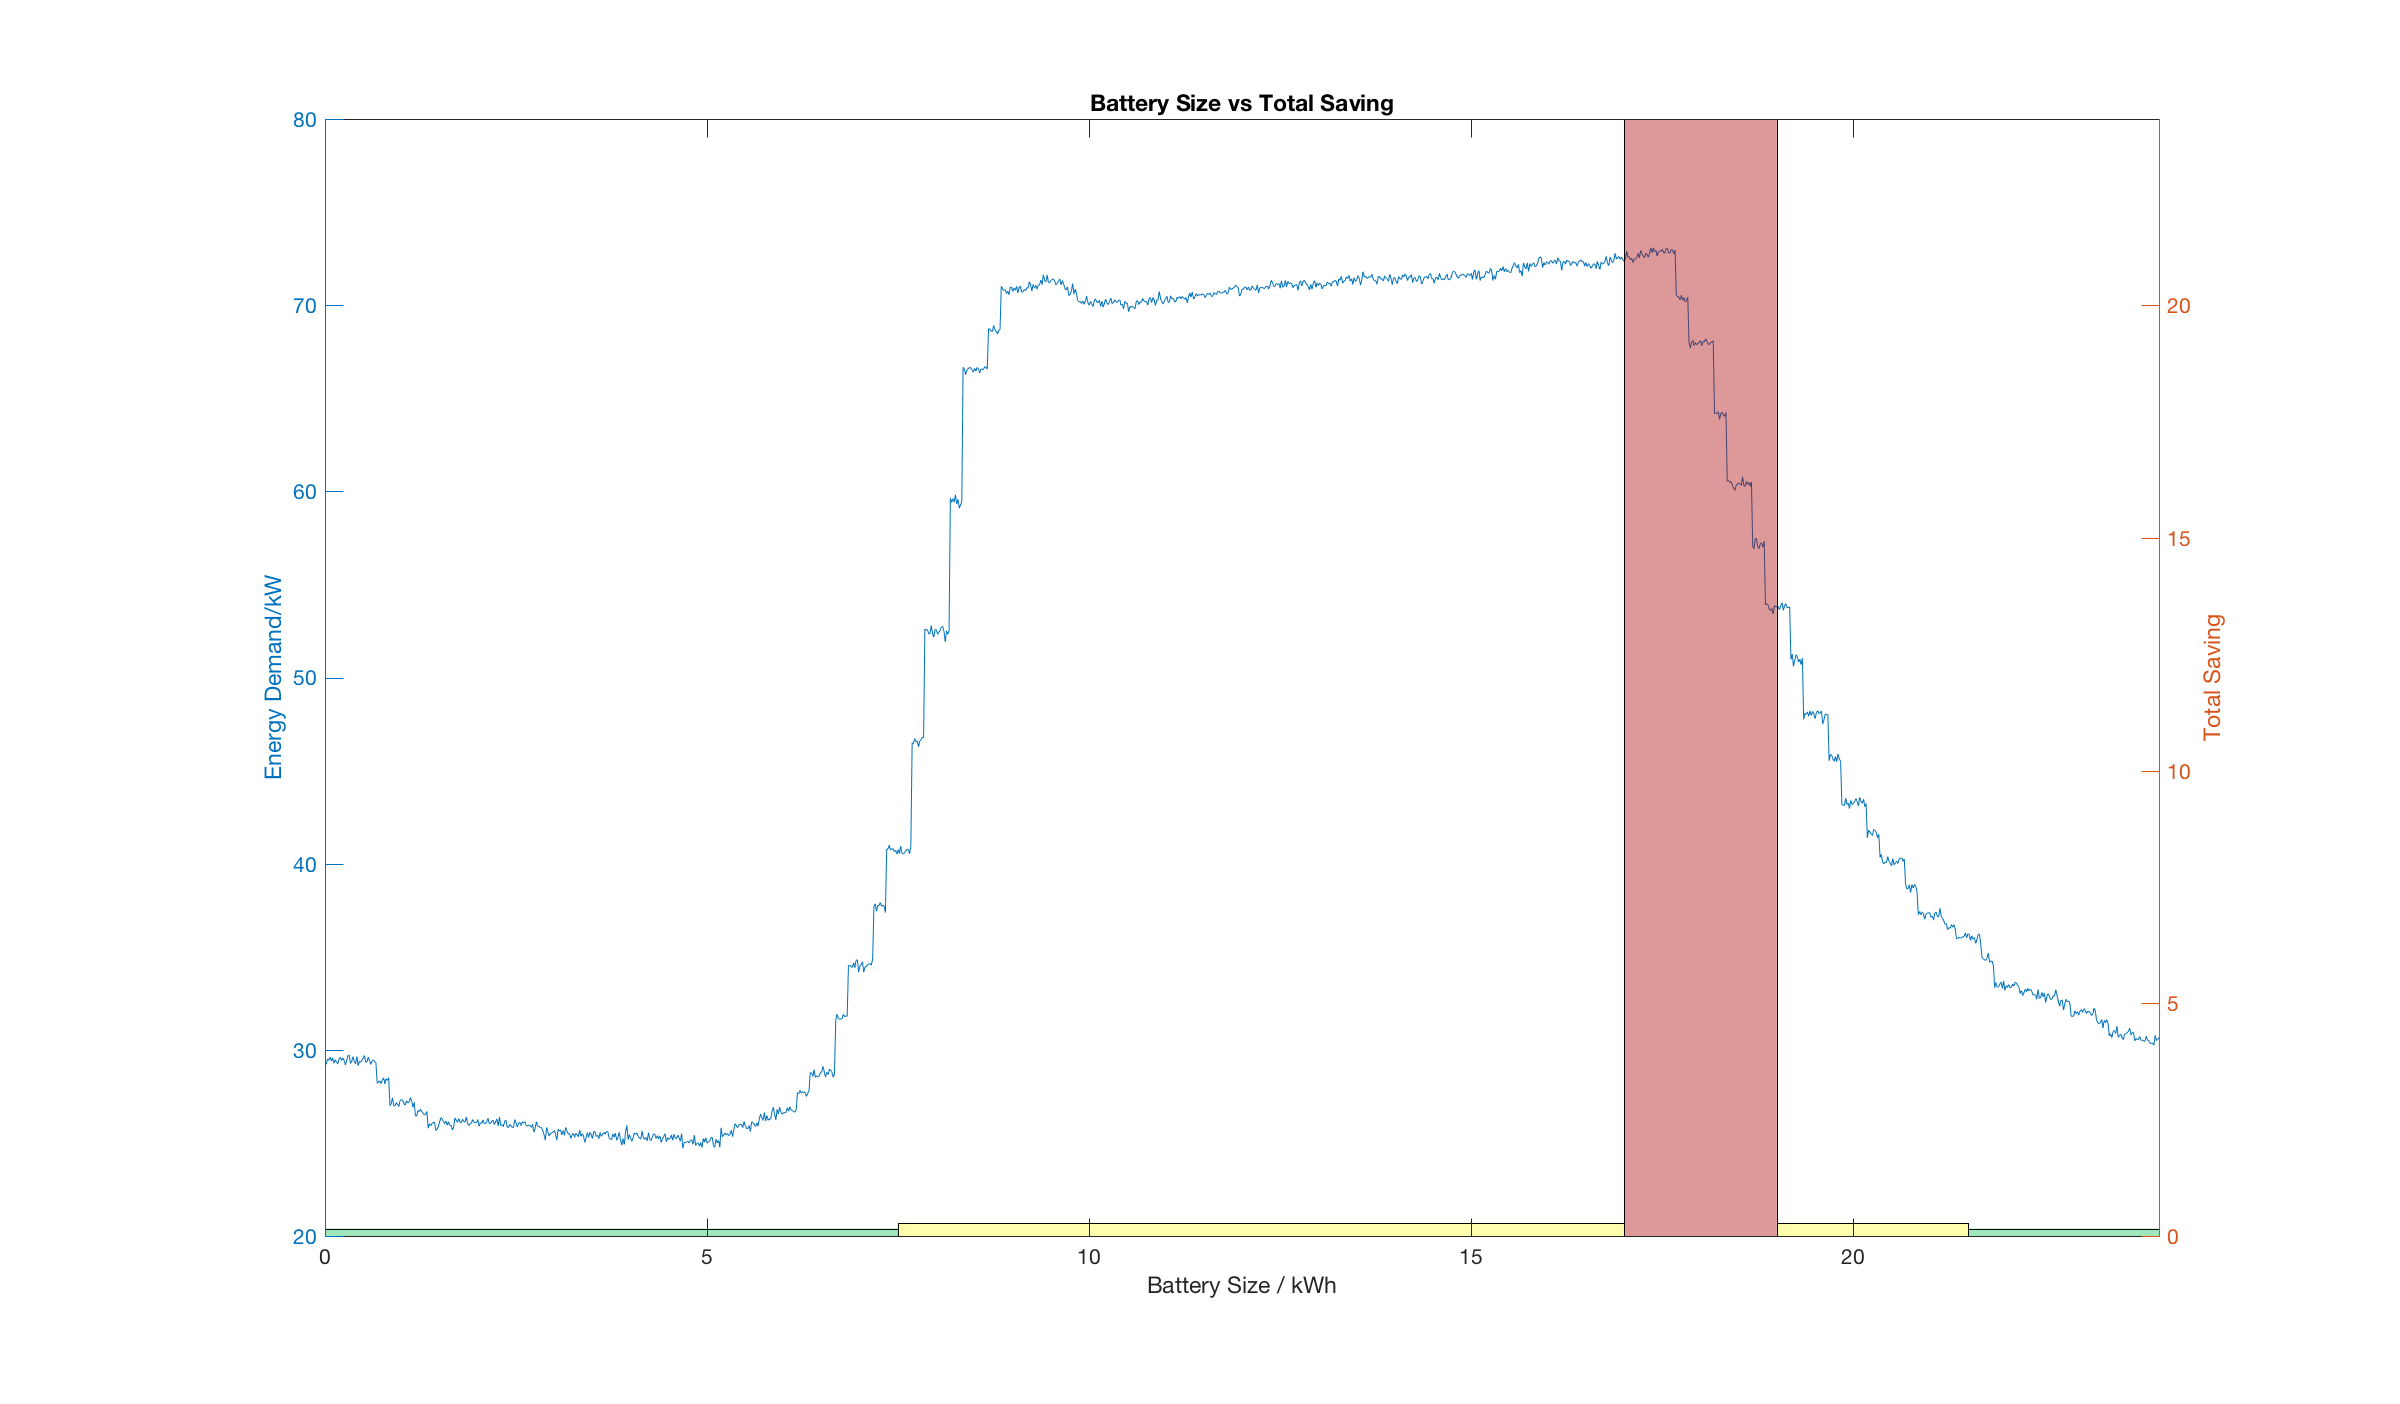
\includegraphics[trim = 0 0 0 0, clip, width=0.5\textwidth]{Development-50.eps}
 \caption{Difference in Unit Charge Rates}
 \label{Development-50}
 \end{figure}

Using this data a model was created taking into account DUoS charges and
multiplying them by their respective rate. This charge makes up and
large \% of the total bill showing roughly how much the unit rate costs.

To achieve this, the date of the usage data was scanned to find which
day the bill began, then assigning the next 6 days, to be either
weekdays or weekends. This was important as there are different DUoS
rate at different times of day between weekdays and weekends. Creating a
counter that loops through each half hour period, logic can be applied
to categorise each half hour period into their respective unit rate.
Total units consumed in red, amber and green periods were found allowing
for some simple calculations to find the effect of load shifting. By
shifting the load in red units to green rate charges, a significant
saving could be made. By measuring the amount of units consumed in red
periods gave a good estimation for the size range of the battery that
would be required.

\subsection{Representative Demand
Profile}\label{representative-demand-profile}

The second performance parameter of the battery is the maximum power it
can supply, rated in kW. By applying to much load on a battery can
ultimately cause it to fail, severely reducing the batteries cycle life.
As there was no demand data available, a few assumption had to be made
in order to generate an valid demand profile. First the half hourly
usage data was split into a minute by minute representation, creating
points at every minute by finding the gradient and constant between two
points then splitting the distant into 30 equidistant points. This
produced an identical graph to the fit, applied by Matlab. However as
each point int he original graph represented usage for the previous 30
minutes, this was divided by 30 to give the usage per minute This can be
validated by summing all the points and compare to the original graph.

This profile however assumes that all usage varies linearly between time
periods. In reality this is not true. To generate a more realistic
demand profile. The start, end and midpoint between two values were used
as means in which a random number with a normal distribution was applied
to give normally distributed values in intervals of 10 minutes,
modelling how usage varies randomly minute by minute but holding the
trend of the original data. Scaling by two, coverts usage from kWH into
demand KW. This graph was then validated by integrating the area of the
graph and comparing it against the summation of the original data. A
standard deviation \(\sigma\), was then selected which would fairly
represent the change in usage. After trailing with a range of different
scales of data, \(\sigma\) was set to the mean between the average usage
and max usage. This gave a fair, but conservative representation of how
energy usage may look.

\textbf{\emph{Assumptions:}} Usage will have a peaky profile due to a
large number of people in the buildings , switching numerous devices on
and off frequently. For an office style building like Senate it is
unlikely that there is any large equipment that could cause a major
spike in demand.

The demand profile could then be plotted as both as histogram and as a
cumulative distribution plot, identifying the typical demand of Senate
house over the year, as well as the max demand the building experiences.
Figures \ref{Development-dd} and \ref{Development-a8} show the demand
profile of the building.

\begin{figure}[H]
 \centering
 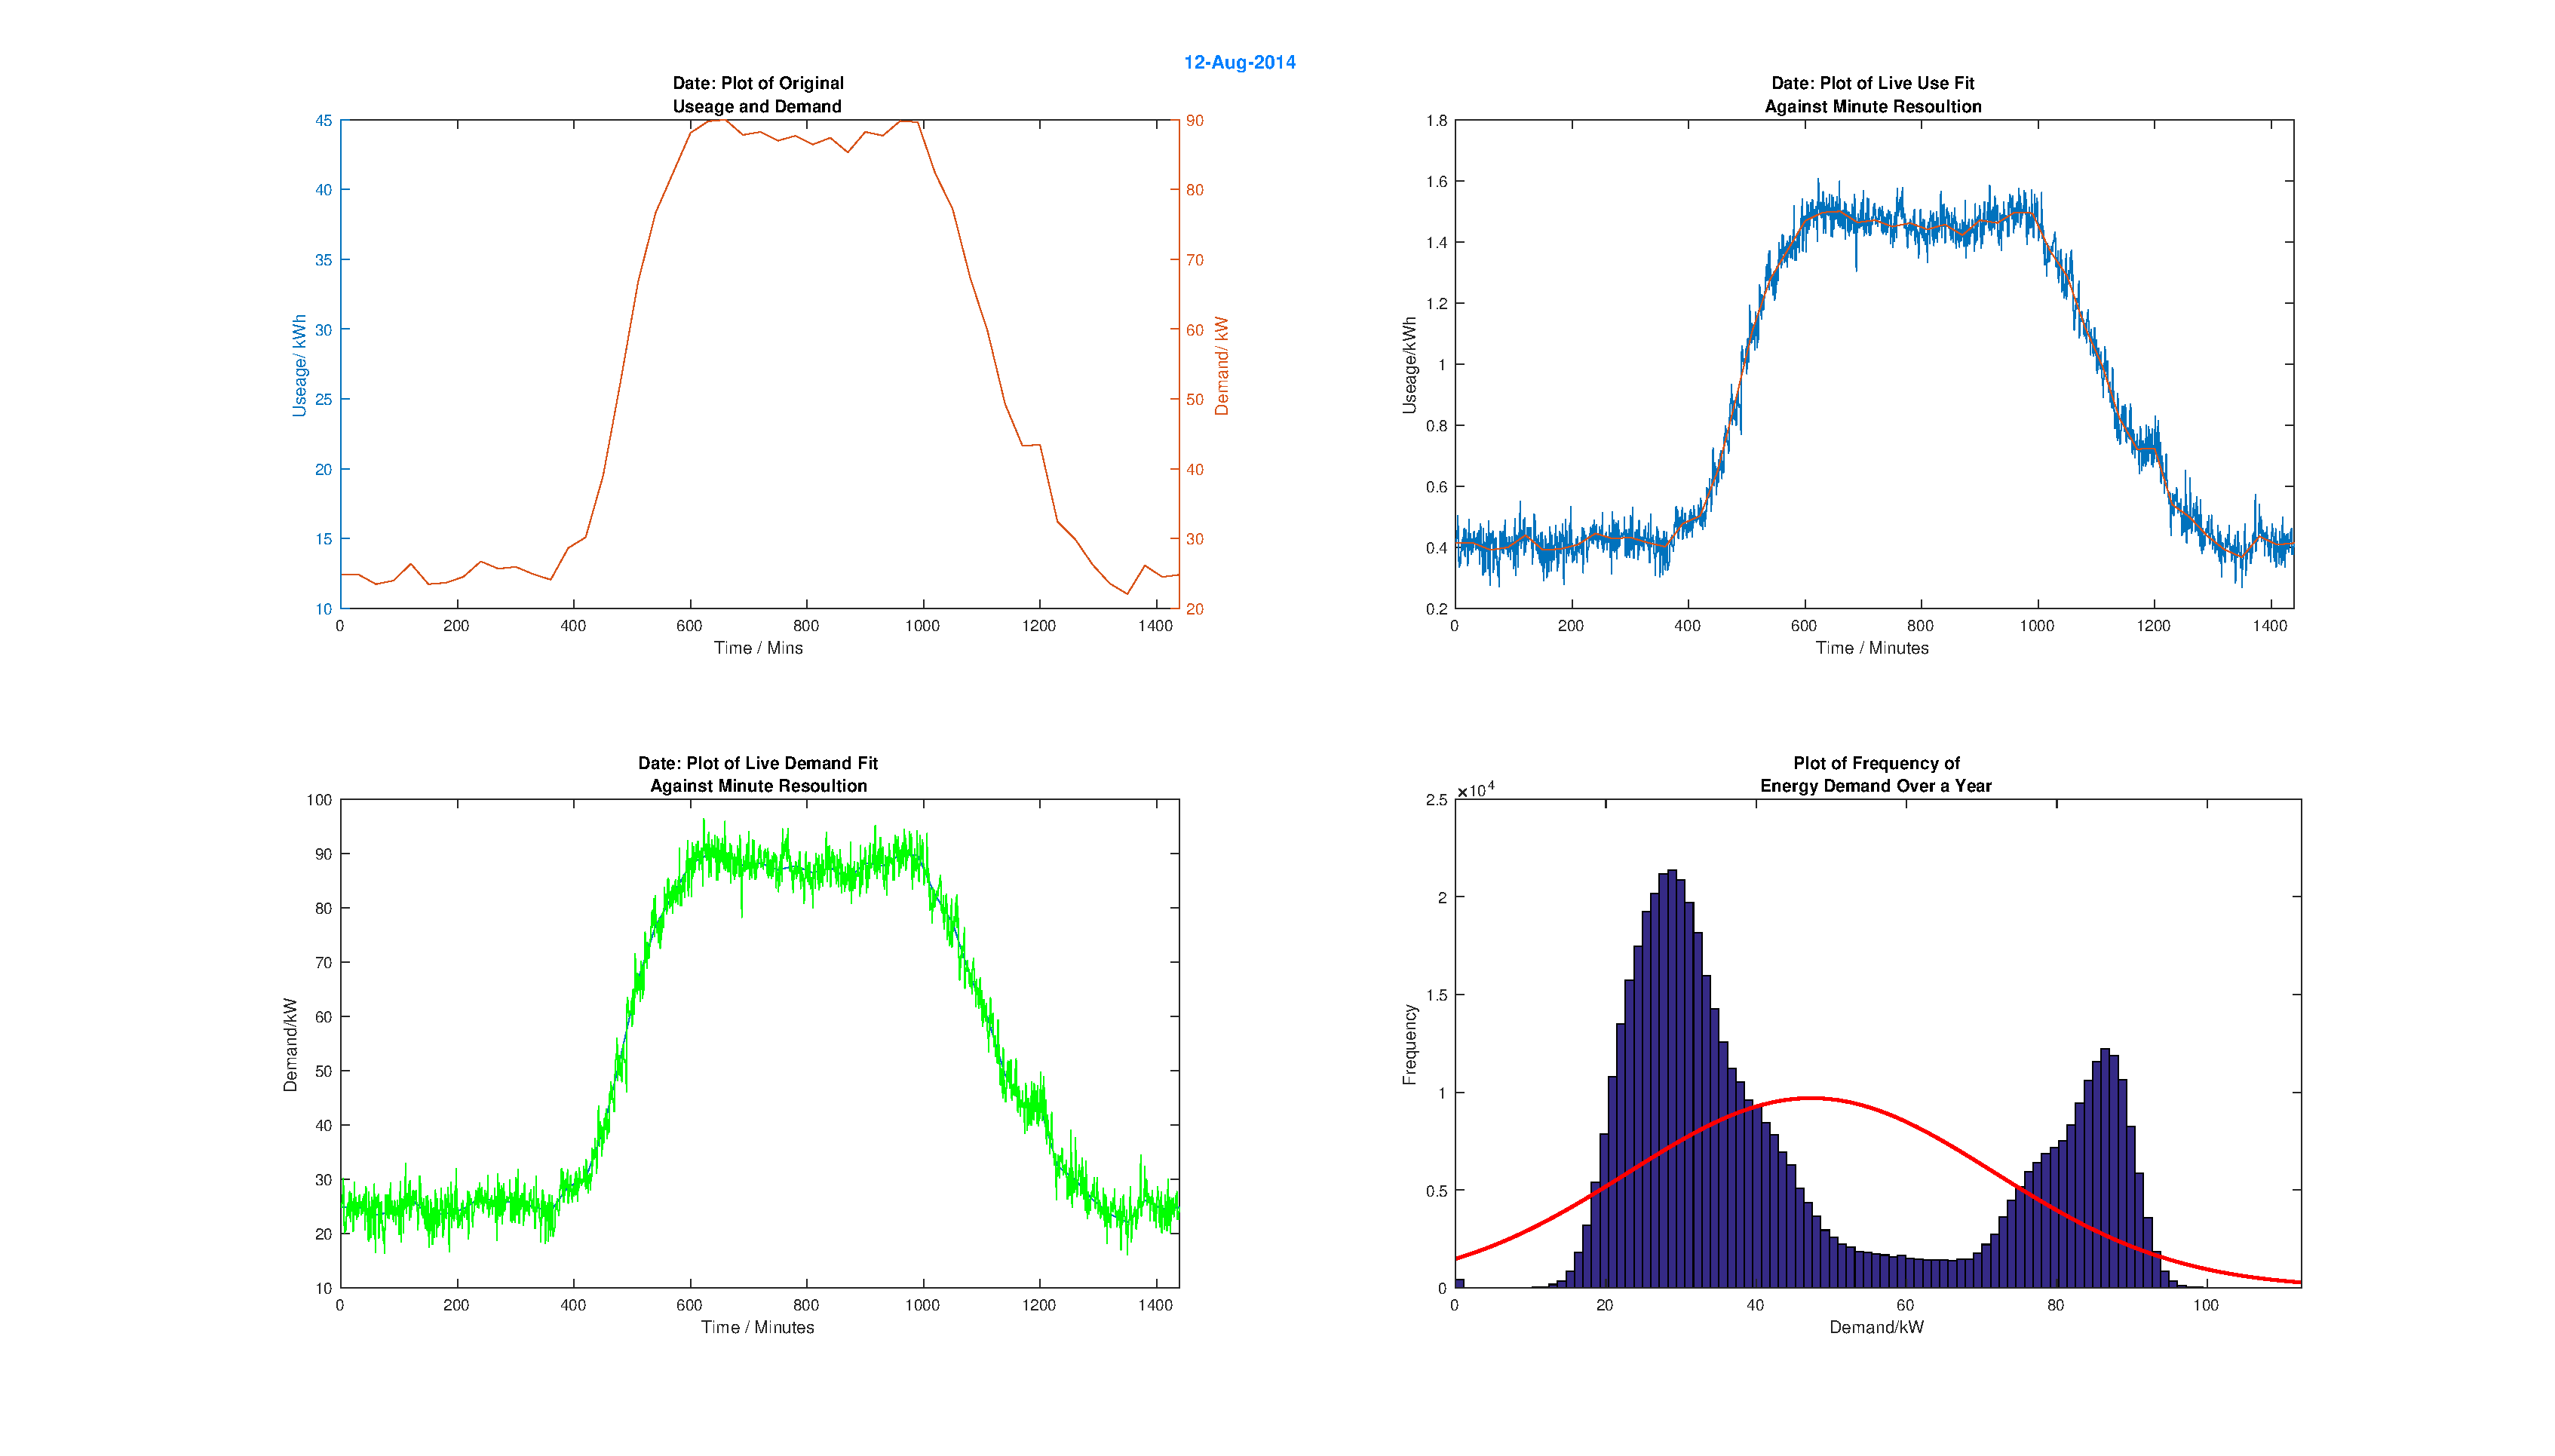
\includegraphics[trim = 140 80 140 20, clip, width=0.95\textwidth]{Development-dd.eps}
 \caption{Plots of Usage and Demand Profile Generation and Histogram of Year Data}
 \label{Development-dd}
 \end{figure}

It can be observed from in the histogram in Figure \ref{Development-dd},
that the demand of the building typically falls between two points. One
low peak representing morning and evening of 30KW and a second peak
constituting the energy usage in the middle of the day, averaging around
80KW, but rarely ever exceeding 90KW.

\begin{figure}[H]
 \centering
 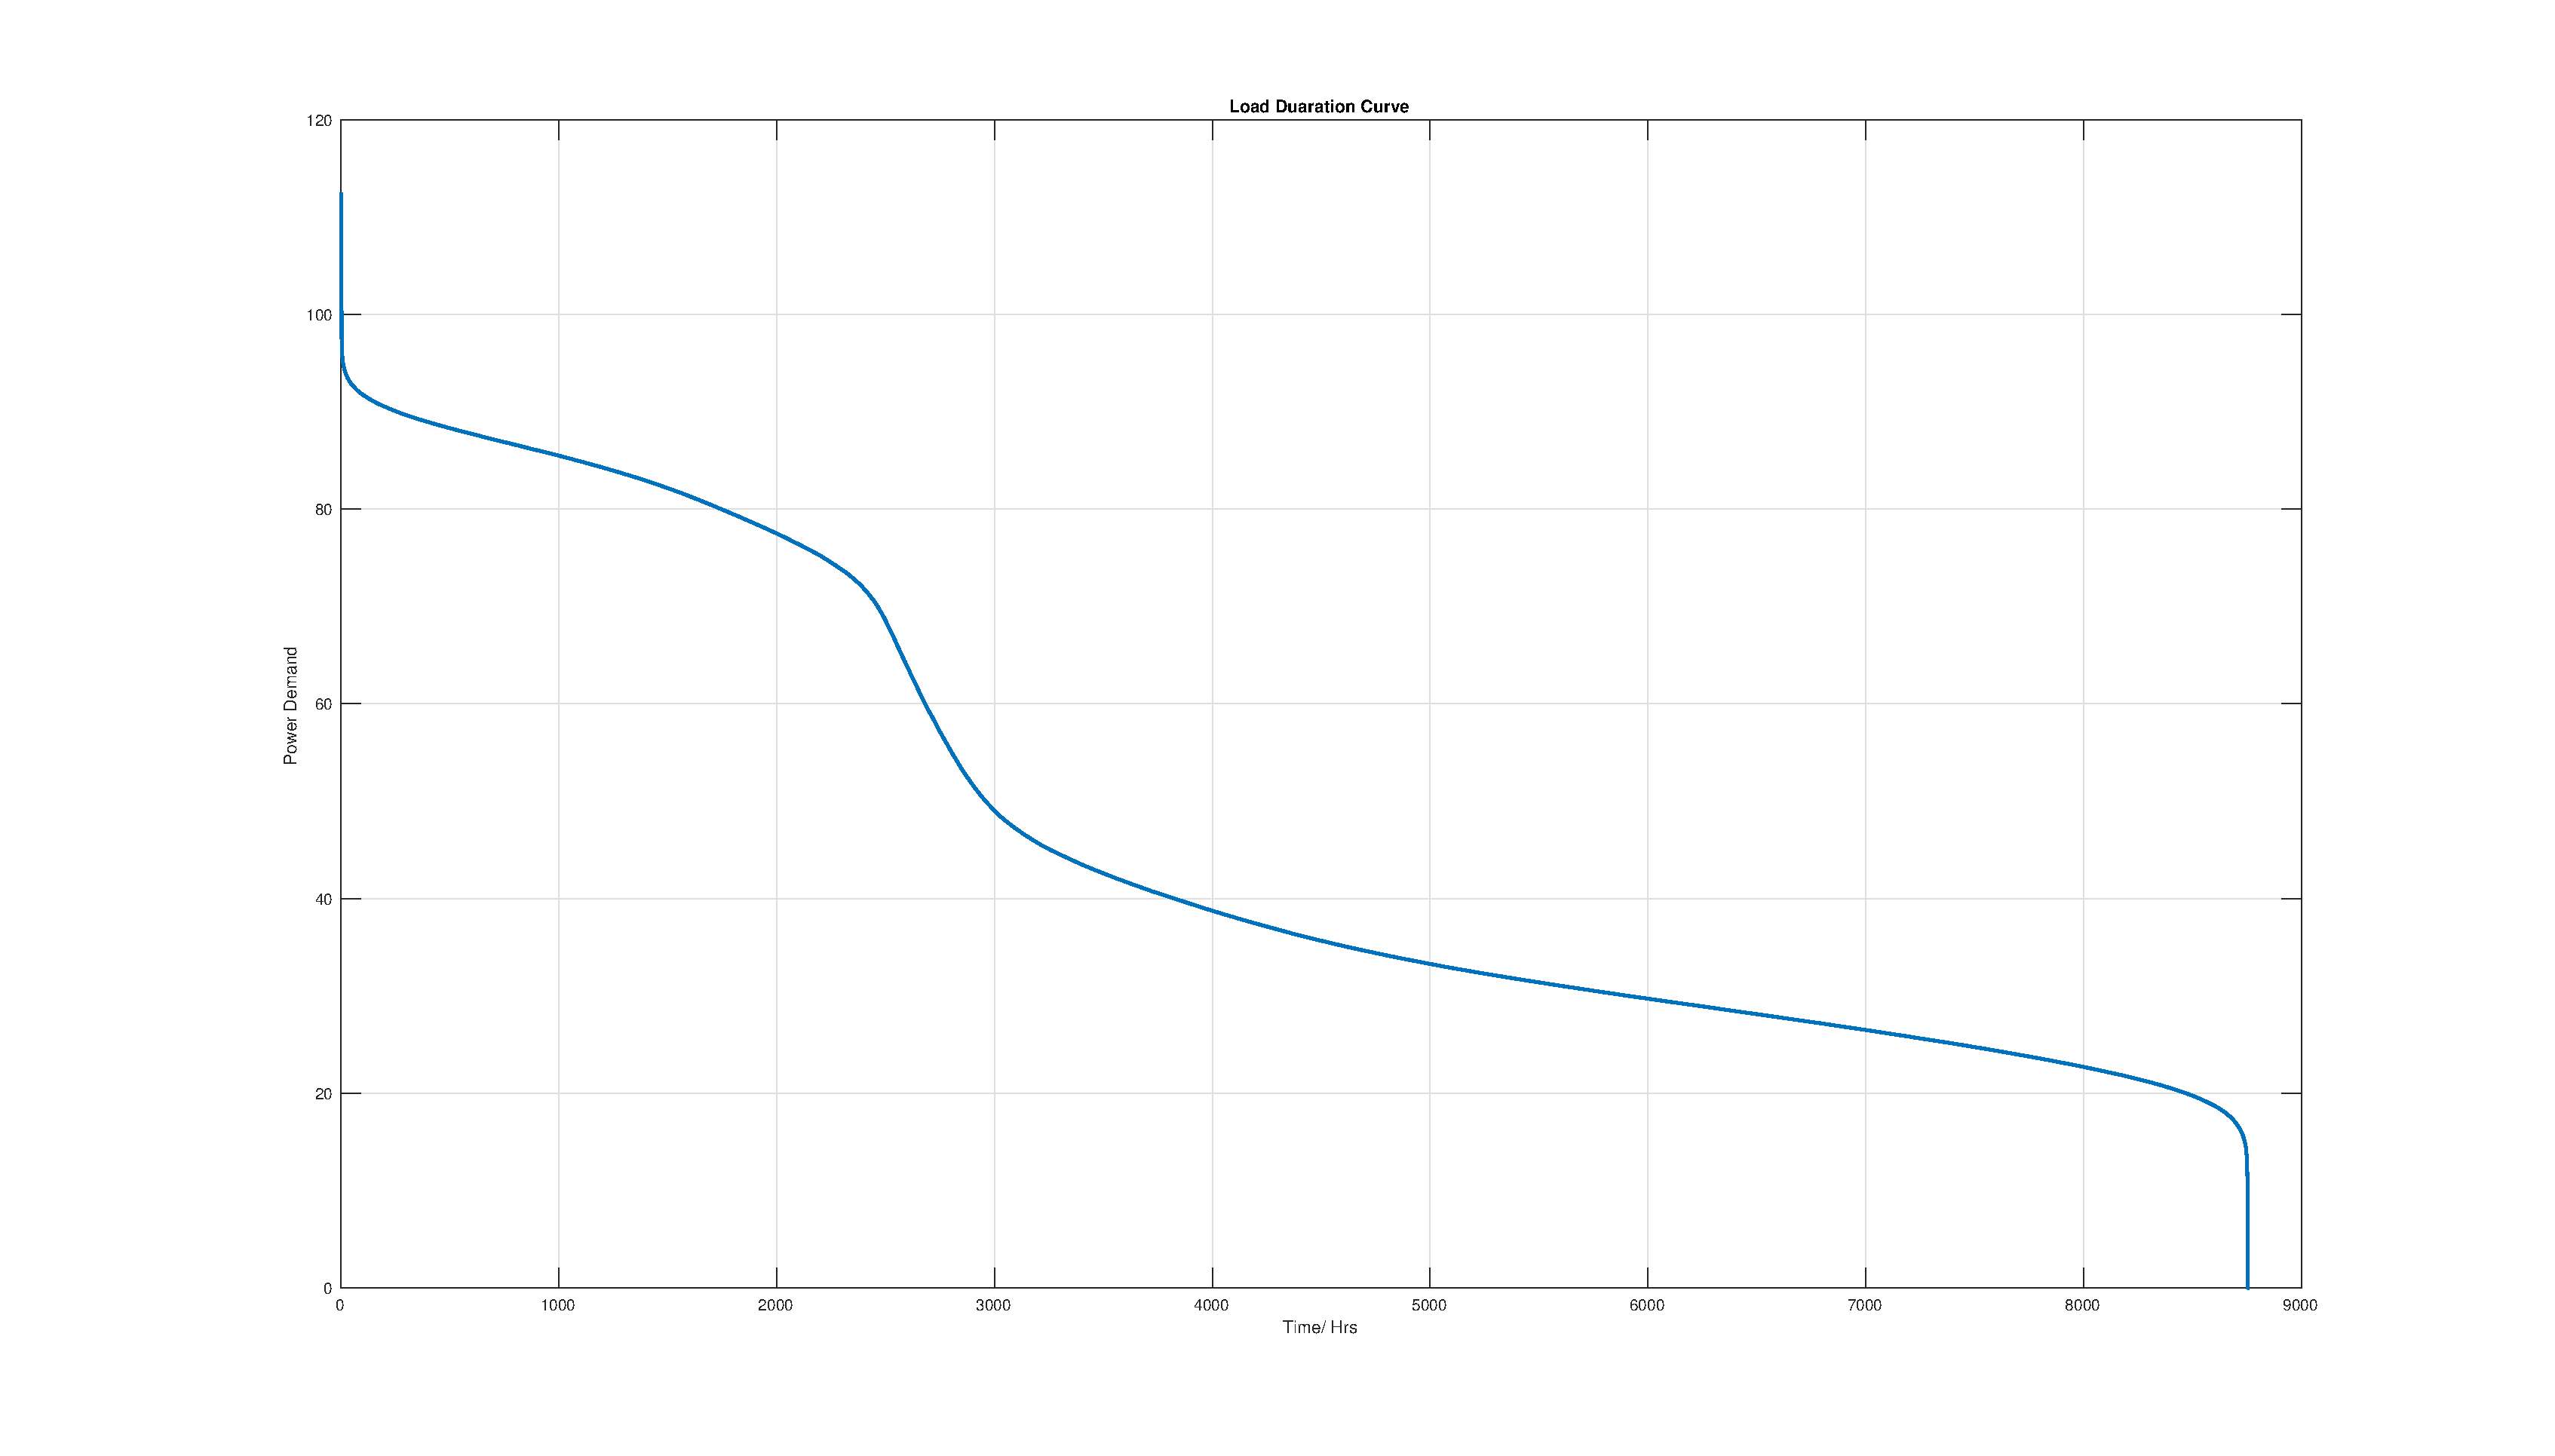
\includegraphics[trim = 0 0 0 0, clip, width=0.7\textwidth]{Development-a8.eps}
 \caption{Load Duration Plot of Year Usage Data}
 \label{Development-a8}
 \end{figure}

The Load Duration Curve in Figure \ref{Development-a8} takes demand for
each hour and plots this in descending order, this shows the annual
demand that can be met for a battery at a given power rating
\autocite{combined-heat-power-buildings}. For Senate house, a battery
rated to 40KW would cover, 5000 hours of the year roughly 55\% of the
years usage.

Taking both graphs together, selecting a battery which covers the mean
power demand, may act be a good trade off.

\subsection{Definition of New Campus
Requirements}\label{definition-of-new-campus-requirements}

To fulfil the objectives of this project, an understanding of the design
of the new campus needed to be assessed. As the building plans are still
in their early stage, many assumptions about the likely size and use of
the campus had to be understood in order to create a representative
energy profile. Table \hl{*Insert Table of campus size/ rooms*} in the
Appendix shows the predicted new campus size and use stating relevant
assumptions.

The campus will constitute around 1500 students in halls of residence
and have around 5000 staff and students on site during term time.
Although there have been a range of facilities proposed that the
University campus will house, it is most likely that the building will
constitute mainly of tutorial rooms, a few lecture halls and offices. A
meeting with John Brenton \autocite{Jbrentmeet}, made clear that
creating infrastucure to support postgraduate business studies made the
most economical sense so is most likely to make up most of the final
plans.

The energy profile of Senate house will be mostly transferrable to the
new campus, as it is unlikely the new campus will have any devices that
will distort the load profile greatly. In addition, the campus is likely
to have improved efficiency through utilising the latest technologies in
its construction and services (ventilation, heating e.c.t.). Data on 125
rooms in halls of residence was also provided, it is likely that this
will almost be identical to a new build, due to student usage making it
difficult to manage energy demand further. Using the foot prints of both
building and adding some additional laboratory data to simulate if these
creates any spike in energy usage.

The scaling factors were:

\begin{itemize}
\tightlist
\item
  Senate House (7840sqm) - \textbf{7.9x}
\item
  Hall data (2761sqm) - \textbf{7.6x}
\item
  Lab data (1 Lab Use) - \textbf{4x}
\end{itemize}

Due to these data files falling under different years and running
between different dates, the data needed to be adjusted in order to be
correctly scaled. An algorithm was therefore created to match the date
shown in figure \ref{Development-fc}.

\begin{figure}[H]
 \centering
 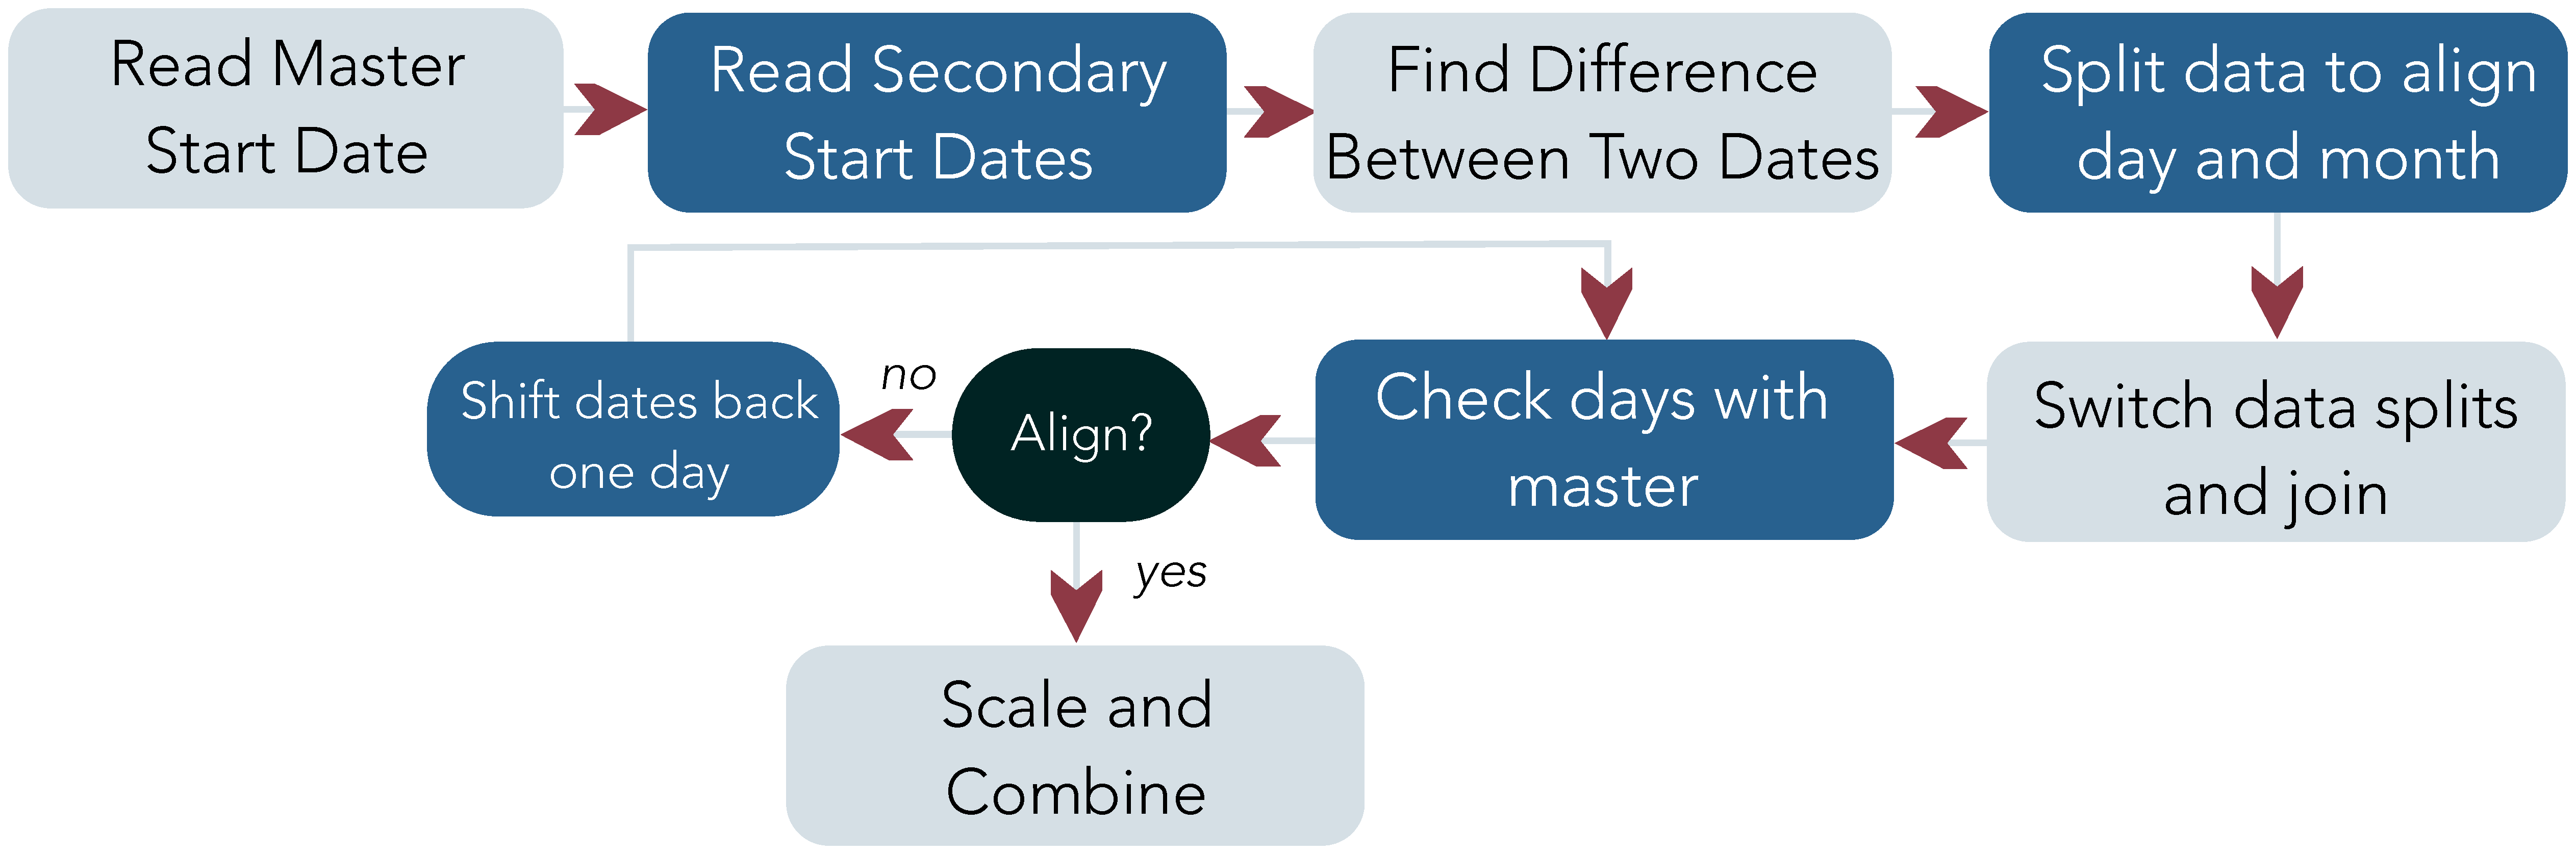
\includegraphics[trim = 0 0 0 0, clip, width=0.9\textwidth]{Development-fc.eps}
 \caption{Logic of Data Aligning Tool To Create New Campus Data}
 \label{Development-fc}
 \end{figure}

\hl{Make assumptions very clear}

\begin{figure}[H]
 \centering
 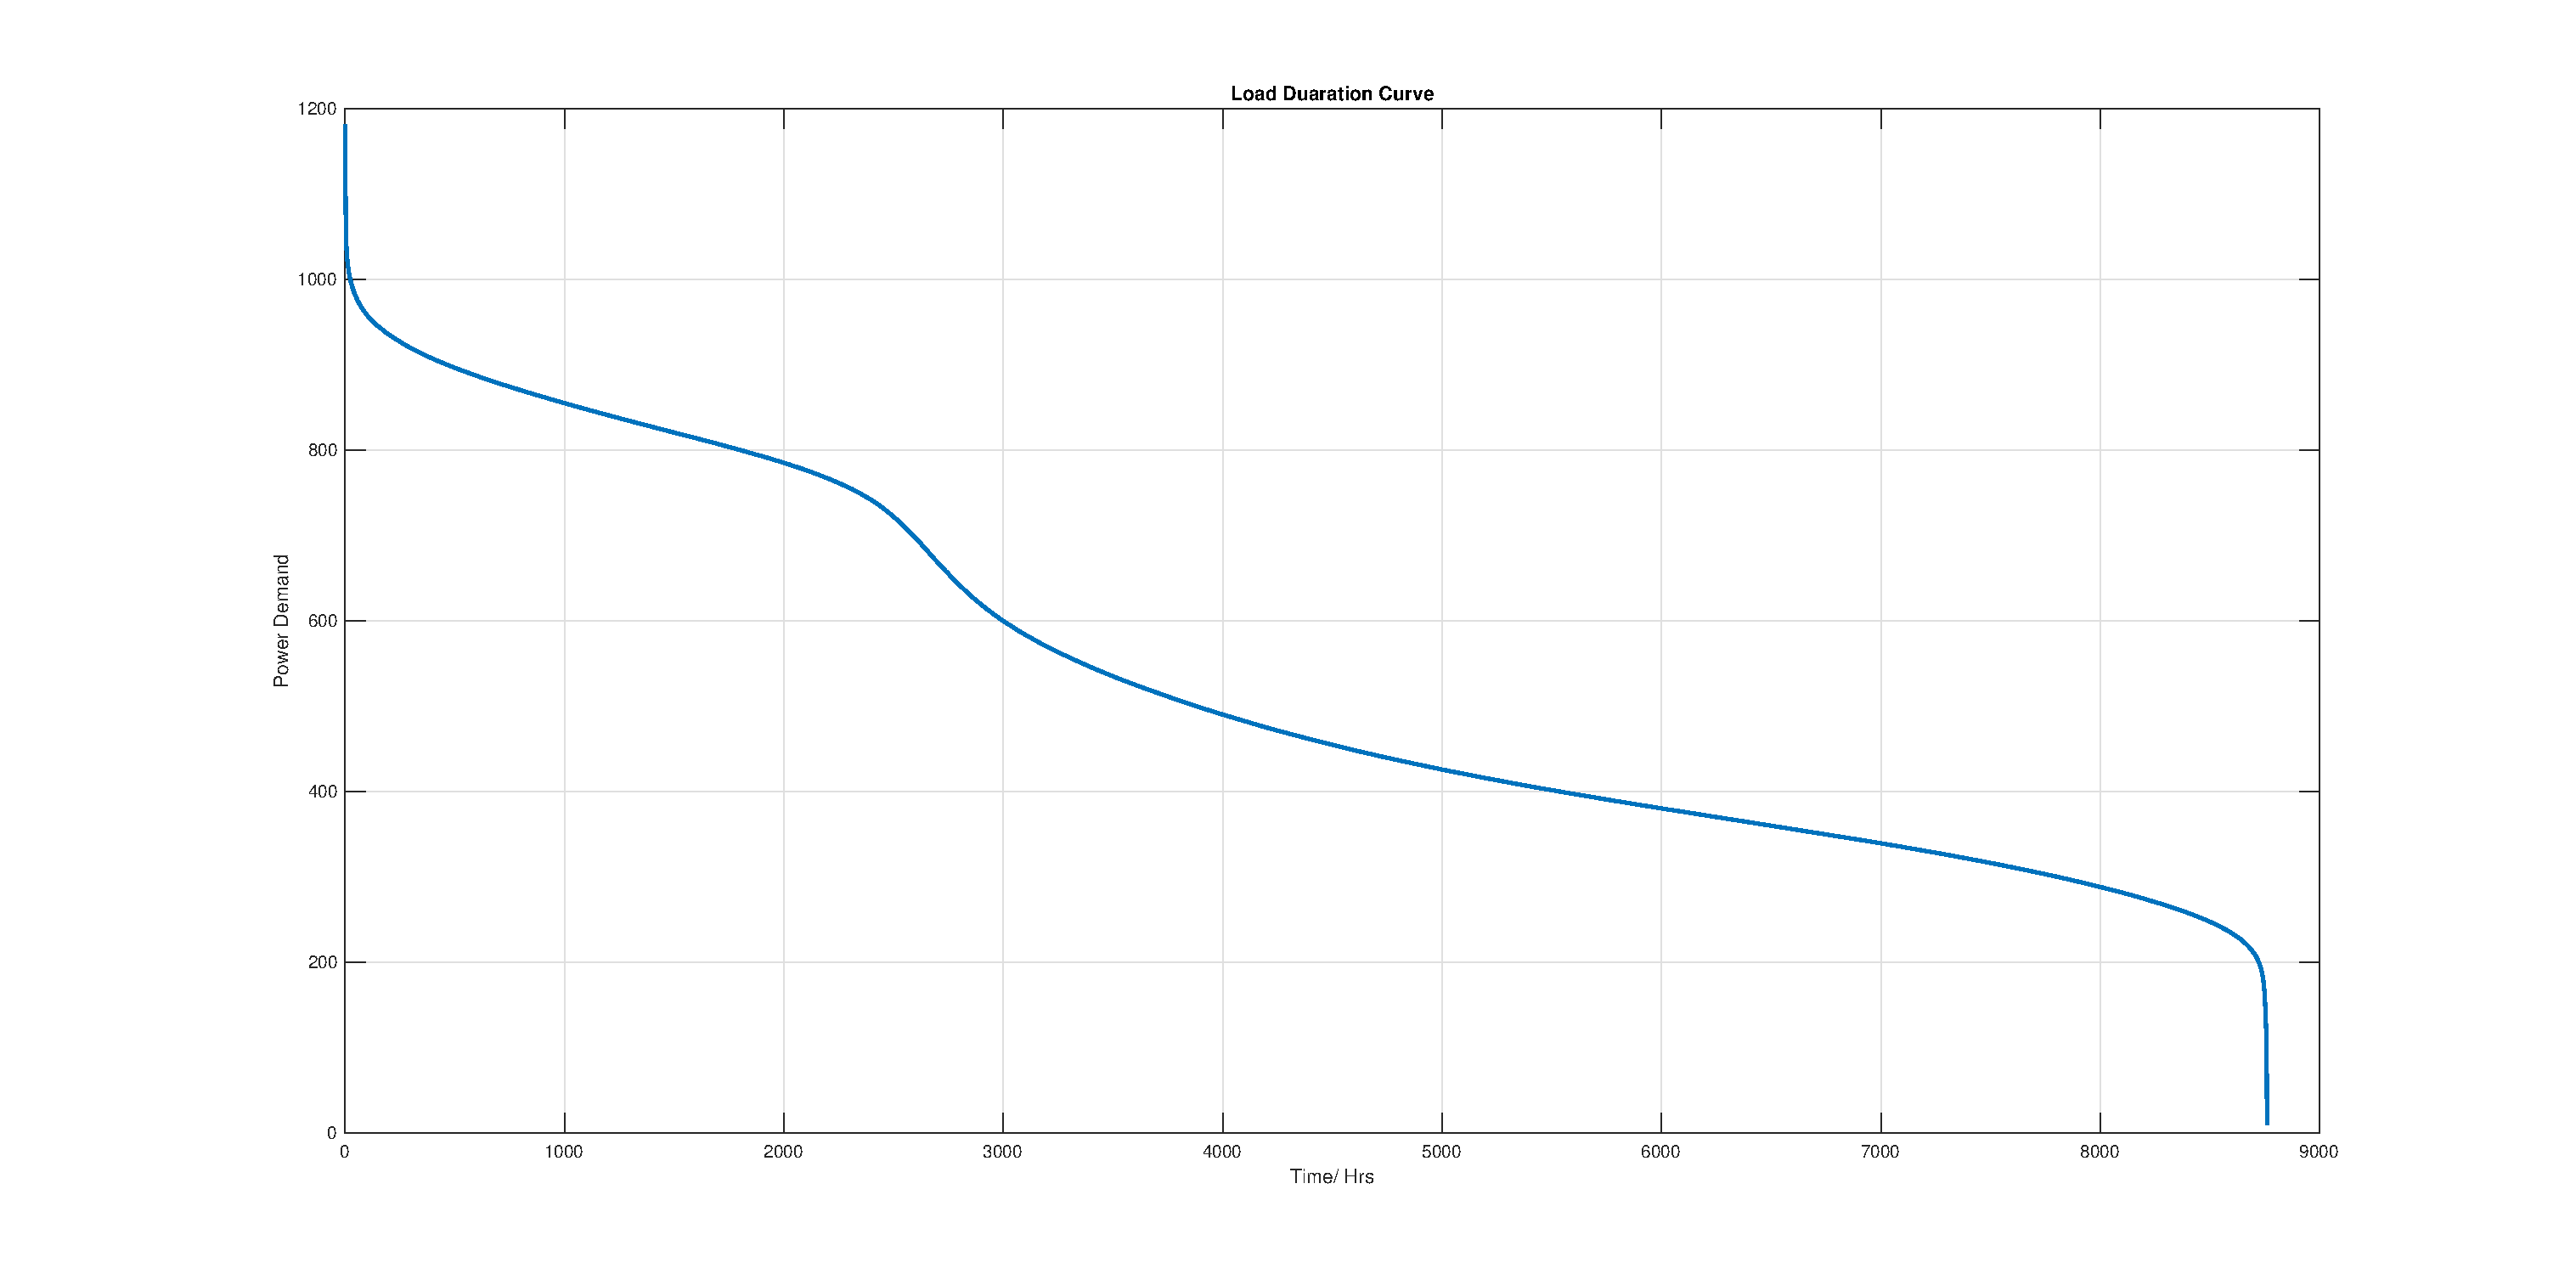
\includegraphics[trim = 0 0 0 0, clip, width=0.6\textwidth]{Development-92.eps}
 \caption{Load Duration Profile for the New Campus}
 \label{Development-92}
 \end{figure}

\subsection{Definition of System Architectures /
Strategies}\label{definition-of-system-architectures-strategies}

Defining how the batteries would run is imperative to understanding
their economic feasibility. This section will define the logic used to
define the operation of the battery and how the model was created to
represent this.

Using the ``live demand data'', created in section
\ref{Representative-Demand-Profile}, a Matlab script was created
simulate through a lifetime use case of the the battery for both Senate
house and the new campus energy profiles. A script was created which
duplicated these data input files for the length of simulation (in
years), checking that each year began on the next day in the week from
the end of the last year. Making sure dates aligned is imperative to
making sure results were valid as the difference in energy usage between
weekdays and weekends, shifts the total savings into a 7 year cycle
pattern. Energy usage and demand data was then run through a second
function which applied three strategies understanding battery
performance from a technical and economical standpoint.

\subsubsection{Red Rate Avoidance}\label{red-rate-avoidance}

As describe in earlier sections, the battery was limited to being
switched on only during red rate periods. This period is always between
5 and 7 on weekdays and has assumed to remain the same for the entirety
of the batteries lifetime. During this period the battery was allowed to
drain itself at a rate up to it's maximum output power. This required
demand and usage data to be checked simultaneously, to make sure the
battery had remaining capacity and was not over loaded. If the load
exceeded its maximum value the supply of energy was capped at this
value. As the battery was used, capacity was decreased proportionally
until live usage exceeded the remaining capacity and the battery was
drained to its minimum capacity and switched off. Or the rate rate
period elapsed.

The battery was then set to begin charging at a set rate when the red
rate period was entered a green rate period. The charging rate was set
based on the amount of charge required divided over the length of the
green rate period. Early discussion of battery life cycle optimisation
suggested that charging at a lower speed, particularly during the last
10\% of charge, made a large impact on the battery lifetime. It is
assumed here that smart charging techniques trickling (seen on most
modern smartphones), would be incorporated into the battery. However the
only value which will effect the outputs of this model is the capacity
when the next red rate period is entered, therefore not necessary in
this model.

This repeats for the run-length of the simulation, measuring the amount
of money saved against the original costs of unit rate charges.

\subsubsection{Triad Avoidance}\label{triad-avoidance}

To correctly understand the effects of TRIAD avoidance in the model, the
dates correlating to each day needed to be correctly applied and matched
against corresponding days. Using \autocite{triad15}, the dates:
4/12/14, 19/01/15, 02/02/15 were used as aligning with the original
Senate data used as a master for the new campus. These dates were used
for the sequential years for days TRIADS would likely fall. Their
corresponding days of the week were checked to make sure they did not
fall weekends and adjusted accordingly if found to be the case. It is
assumed here that daily variation in energy usage is negligible and
instead energy trends are seen only on a monthly basis. This means that
it does not matter if the TRIAD lands on a Monday or a Friday, and
instead the date corresponds best with predicted weather pattern- the
only variable likely to cause observable differences on a calendar data
(any other variables have been ignored, particularly as these will
cancel out over time).

These periods were all between 5 and 7 corresponding with the battery
strategy already in place. Using these dates and the time of 5:30, the
TRIAD cost was calculated based on energy demand at this time. Battery
usage was then measured against the TRIAD cost to understand the
reduction in energy demand delivered by the battery. The reduction in
TRIAD rate was a factor of the batteries max power supply and not
capacity. As the battery would only need to run for a few minutes to
offset this charge.

At the end of each year in the simulation the three TRIAD costs were
averaged to find the total cost. This was then spread evenly over the
next year in the simulation, representing how TRIAD billing is split
across each monthly energy bill.

\subsubsection{Battery Degradation
Modelling}\label{battery-degradation-modelling}

As highlighted in section
\ref{battery-lifetime-assessment---understanding-battery-degradation}
discusses the different variables which can effect a batteries cycle
life. An approximation of the batteries was taken, taking into account
the effect of each of these variables and placing a battery usage
strategy in place. The rated battery cycle life is taken to be the
number of full cycles a battery can complete before it has degraded to
80\% of it's original capacity. This figure was used as it is the best
metric for how a battery should perform based on a normal use case. The
model uses this assumption to degrade the battery by the fraction of
it's cycle life that it has charged up by. For each charging iteration
the new max capacity becomes slightly smaller, reducing the size of the
cycle. A counter is then run summing up the amount the battery has
charged. When this equals the current maximum, a complete cycle has been
fulfilled. The effect of this method means that the battery will degrade
faster the longer it has been applied. This follows the mean trend of
battery cycle life shown in figure \ref{batCapGen}.

Any assumptions made about battery degradation were based on battery
operation and not the batteries chemistry. Assumptions were made on what
constitutes ``normal working parameters'', alleviating extremes in modes
that have an exponential effect on how the battery degrades. To reduce
wear on the battery, the battery was confined to work within 10-90\% of
it current maximum capacity, allowing a maximum depth of discharge of
80\%. Draining the battery can cause detrimental effects on the whilst
overcharging can also do the same. Working within these two parameters
follows similar principles applied by Tesla in their electric cars
\hl{add reference here}. The battery was never run above it's demand
maximum (max power KW), however no factor was used to degrade the
battery quicker if it operated at this factor (a known cause of wear).
As the battery was rated at this value, it should be designed to cope at
this level of use for no longer than 2 hours a day.

Temperature was also assumed to remain within expected bounds. Britain
only experiences hot days a few times a year and rarely drops below
freezing, making it a better climate for battery operational
temperatures than the states where average temperatures are a lot
hotter. Using the two strategies defined above means the battery is only
ever discharging or charging 5 days a week, with some charge on a
Saturday mornings dependent on the battery selected. This allows the
battery too cool down and perform any life enhancing cycling activities
if relevant
\hl{Consider how these two days could be used to improve the batteries lifetime}.

The model was run until either the runtime reached it's end or the
battery reached it's end of life value of 80\%. This meant answer were
comparable. It is worth noting that there are examples of batteries
being used beyond their end of life cycle.
\hl{This is being seen by Nissan/ Honda in recycling their car batteries to use in homes},
as there are little associated costs with batteries after they have been
installed if the battery has payed itself back, the battery will
continue to generate profit. However as there is a lot of
unpredictability about whether the battery will fail, this has not been
regarded in the model and instead seen as the asset no-longer holding
any more value.

\hl{Diagram of Battery Cycling Degradation}

\subsubsection{Battery Efficiencies}\label{battery-efficiencies}

Battery efficiency was regarded in the model by multiplying the energy
drawn when charging by the additional loses caused inefficiencies. This
assumptions was made as it is likely that the battery once charged can
supply what it has stored, although some losses will be incurred when
transforming back to AC again. It is assumed that the efficiency figure
regards both transformations. Efficiency gains could also be achieved by
designing the system so it primarily sends power to DC first without
transforming. Efficiency however does not play a huge part in improving
costs savings due to the difference between charging in green periods
and the red rate being so significant.

\subsubsection{~Input Parameters and Multi-Battery
Simulation}\label{input-parameters-and-multi-battery-simulation}

In order to understand the optimum battery type for a given scenario,
and then infer the total savings that the battery could generate; a
large array of different batteries with different power ratings and
capacities was modelled. This required iterating the model numerous
times. To reduce computation time, parallel computing was implemented to
iterate each discrete battery scenario in the 0D model.

The following Operational Parameters Were Used to Generate the Output
Results Discussed in this report. Values stated as variables were varied
per battery.

\begin{table}[H]
\begin{tabular}{p{4.3cm}p{8cm}}
\textbf{Upfront Costs}:& Variable\\
\textbf{Max Power}:& Variable\\
\textbf{Upfront Costs}:& Variable\\
\textbf{Depth Of Discharge \textit{(DoD)}}:& 80\% \\
\textbf{Cycle Life}:& 5000 [@TeslaPow57:online]\\
\textbf{Max Charge}:& $\frac{1-\text{DoD}}{2+\text{DoD}} \times$ CurrentCapacity\\
\textbf{Min Charge}:& $\frac{1-\text{DoD}}{2} \times$ Current Capacity\\
\textbf{End Life Value}:& 80\%\\
\textbf{Additional Costs}:& £0 \\
\textbf{Charge Rate}:& Max Power $\times$ 0.4 (In kWh per Half Hour)\\
\textbf{TRIAD Days}:& 04-Dec-2014, 19-Jan-2015, 02-Feb-2015\\
\textbf{TRIAD Rate}:& £33.55  (price per KW)\\
\textbf{Unit Rate}:&  6.832p\\
\textbf{Red Rate}:&  24.41p\\
\textbf{Amber Rate}:&  0.287p\\
\textbf{Green Rate}:&  0.161p\\
\textbf{Usage Variation $\sigma$}:&  $\frac{\text{Max Value + Mean Value}}{2}$ (For minute by minute granularity)
\end{tabular}
\label{inputparam}
\caption{Table Showing the Input Parameters of the Model}
\end{table}

The following diagram depicts the model of the entire multi-battery
system.

\hl{Large system Diagram of the Logic behind the model}

\hl{It was important that the model was as clear and simple as possible. To improve clarity within the model, structures were used to group variables. The benefit of using structures is the ability to pass them into a function. Using structures throughout the Lagoon Energy Model function and Multiple Lagoon Model script allowed all the required variables to be passed between the function and script using one structure. This greatly improved the structure and clarity of the model script.}

\subsection{Performance Optimisation of Battery Storage
Model}\label{performance-optimisation-of-battery-storage-model}

\autocite{getreuer5685writing}

\begin{itemize}
\tightlist
\item
  Use Profiler
  \hl{Within MATLAB, the performance of a code can be measured in the amount of time it takes to run. The MATLAB profiler is a useful tool which records the amount of time spend in the different functions called within a script. The profiler can be used to identify bottlenecks within the model.}
\item
  Array Preallocation
\item
  Vectorisation
\item
  Reference Wildcards
\item
  Delete Sub Matrices
\item
  Convert to column vectors
\item
  Parallel Computing For loops
\item
  Minimised using MATLAB functions (linear interpolation etc.)
\item
  Used single instead of double integers (half size of memory
  allocation).
  \hl{The default storage method for data within MATLAB is a double-precision floating point number (Mathworks, 2016). This method of representing a number within CPU memory is able handle very large values, however requires 64 bits per number. By storing numbers as a single-precision data type, only 32 bits are required, reducing the data size by a half. This helps to manage memory within the model.}
\item
  DRY coding technique
\end{itemize}

\section{Validation of Model}\label{validation-of-model}

\subsection{Data File}\label{data-file}

By using the model with real data first taken from Senate house, the
tool which creates live data could be validated through integration and
direct comparison to the original usage data. As no data could be
gathered on how the demand profile looks for Senate house, assumptions
were made on the type of operations the building fulfils (see the table
below); this was compared to demand data at Princeton
\autocite{LiveData90:online}.

\subsection{Model}\label{model}

\hl{ADD Model validation thoughts, short as Assumptions hope to capture why the model is valid based on what has been used, validation table (excel) place simple calculation in body, additional thoughts on sensitivity analysis}

\subsection{Limitations / Assumptions}\label{limitations-assumptions}

\hl{Create Full Table of Assumptions - ADD TOO HERE}

\begin{itemize}
\tightlist
\item
  Office buildings are unlikely to have highly peaky demand profiles as
  there is no large devices that could cause spikes
\item
  Red rate times remain the same for the entirety of the batteries
  lifetime
\item
  Normal distribution of energy demand between each half hour period

  \begin{itemize}
  \tightlist
  \item
    Sigma = average between mean of data and max of data
  \end{itemize}
\item
  Trickle charging and minimum charge rate employed
\item
  Daily Variation- negligible

  \begin{itemize}
  \tightlist
  \item
    Other variation in energy use ignored
  \item
    Weather the only contributor worth noting
  \item
    TRIAD dates kept as close as possible to the original (no
    weekends)\\
  \end{itemize}
\item
  Battery operation assumptions
\item
  Does not overheat
\item
  Run within normal working parameters
\item
  Battery chemistry assumptions

  \begin{itemize}
  \tightlist
  \item
    Cycle life rating of battery indicates degradation in normal use
    case
  \end{itemize}
\item
  Battery efficiency losses lost on charging

  \begin{itemize}
  \tightlist
  \item
    Figure quotes both battery transformation
  \end{itemize}
\end{itemize}

\section{Results}\label{results}

This project aims to evaluate whether the value gained from purchasing
batteries outweighs its large upfront costs and other challenges that
battery technology faces. This section analyses the data gathered from
zero-dimensional model and discusses the plausibility of using a battery
and which battery is optimum based on a demand profile for both Senate
House and the new University campus.

\subsection{Senate House Battery
Optimisation}\label{senate-house-battery-optimisation}

\hl{
  * Graphs of NPV, Total Savings and Payback Time
  * Discussion on installation costs
  * Optimum battery to choose
}

\subsection{New Campus Battery
Optimisation}\label{new-campus-battery-optimisation}

Using the input values defined in section
\ref{definition-of-new-campus-requirements}, the model was used
generated results for 113 different battery types. Due to the size
demand profile of the battery requiring up to \hl{xkW} in a during a red
rate period, and requiring a capacity of up to \hl{ykWh}, meant that
many different solutions were plausible for providing the most value. By
simulating for a range of batteries over a period of time, key trends
between capacity and max power could be seen. A 25 year period was
selected to evaluate the battery performance over. It is expected that
after this period of time, technology will have significantly changed,
refurbishments on the buildings will be under consideration and
unpredictability on the long term use of the batteries will be reduced.
The following results will talk through the three key value measurements
discussed in section \ref{battery-economics}.

\subsubsection{Total Savings and Payback
Period}\label{total-savings-and-payback-period}

Due to the 25 year limit placed on the batteries, the largest batteries
did not necessarily deliver the greatest savings due to their high
purchase price not being converted into additional savings from the
battery strategies having no further load to be shifted. Figure
\ref{SRTS2} shows the parabolic shape with a local maximum between the
battery size and the total savings for a 25 year period. For the new
campus, a battery size of around 2000 kWh appeared to be the best choice
battery to select. The max power needs to be very high, with a 1.2-1.3
MW power response, to access these maximum total savings.

\begin{figure}[H]
 \centering
 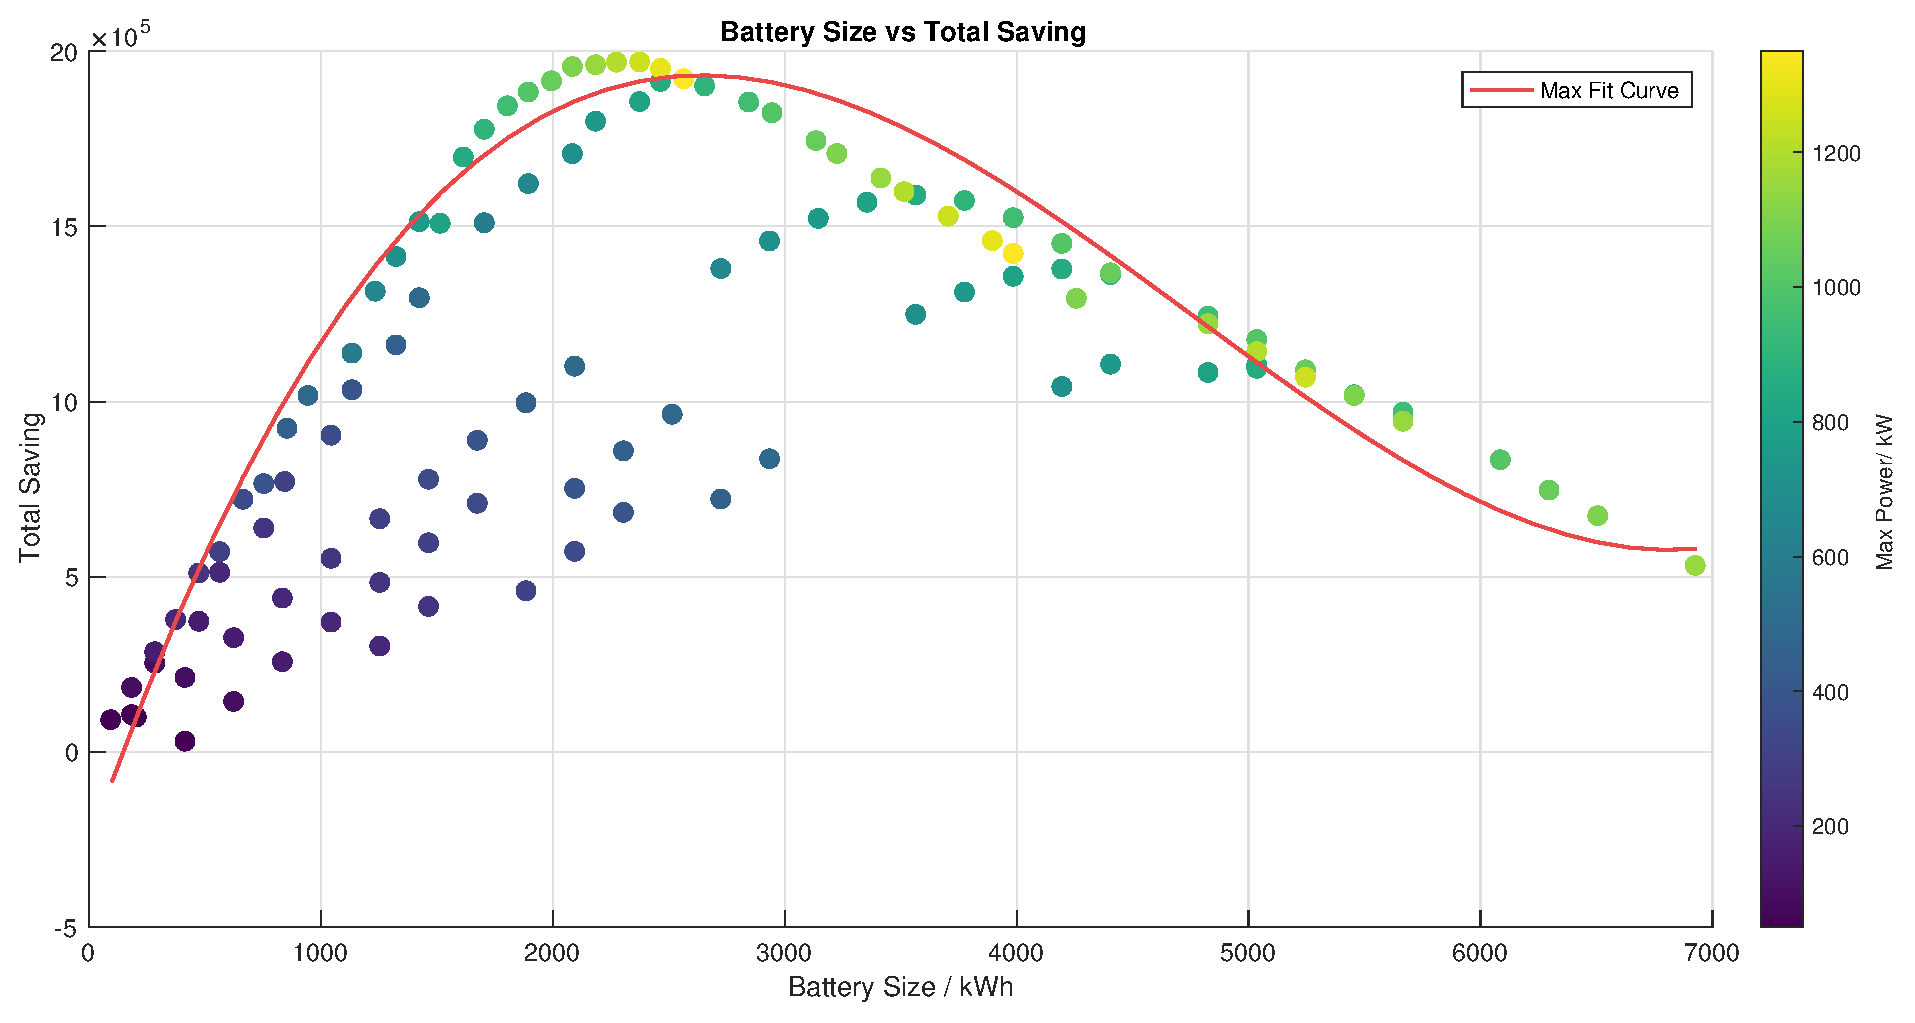
\includegraphics[trim = 0 0 0 0, clip, width=0.7\textwidth]{SRTS2.eps}
 \caption{Battery Size Vs Total Savings}
 \label{SRTS2}
\end{figure}

Looking at the payback period shown in Figure \ref{SRPB2}, a different
story is told. The correct combination of max power and battery size is
required to get a payback period between 6.3 and 8 years. Battery Sizes
all remain below 2000kWh and provided that the battery size is paired
with the correct maximum power, the shortest payback period can be
accessed. After the 2000kWh mark, capacity rather than max power has the
greatest effect in increasing the payback time.

\begin{figure}[H]
 \centering
 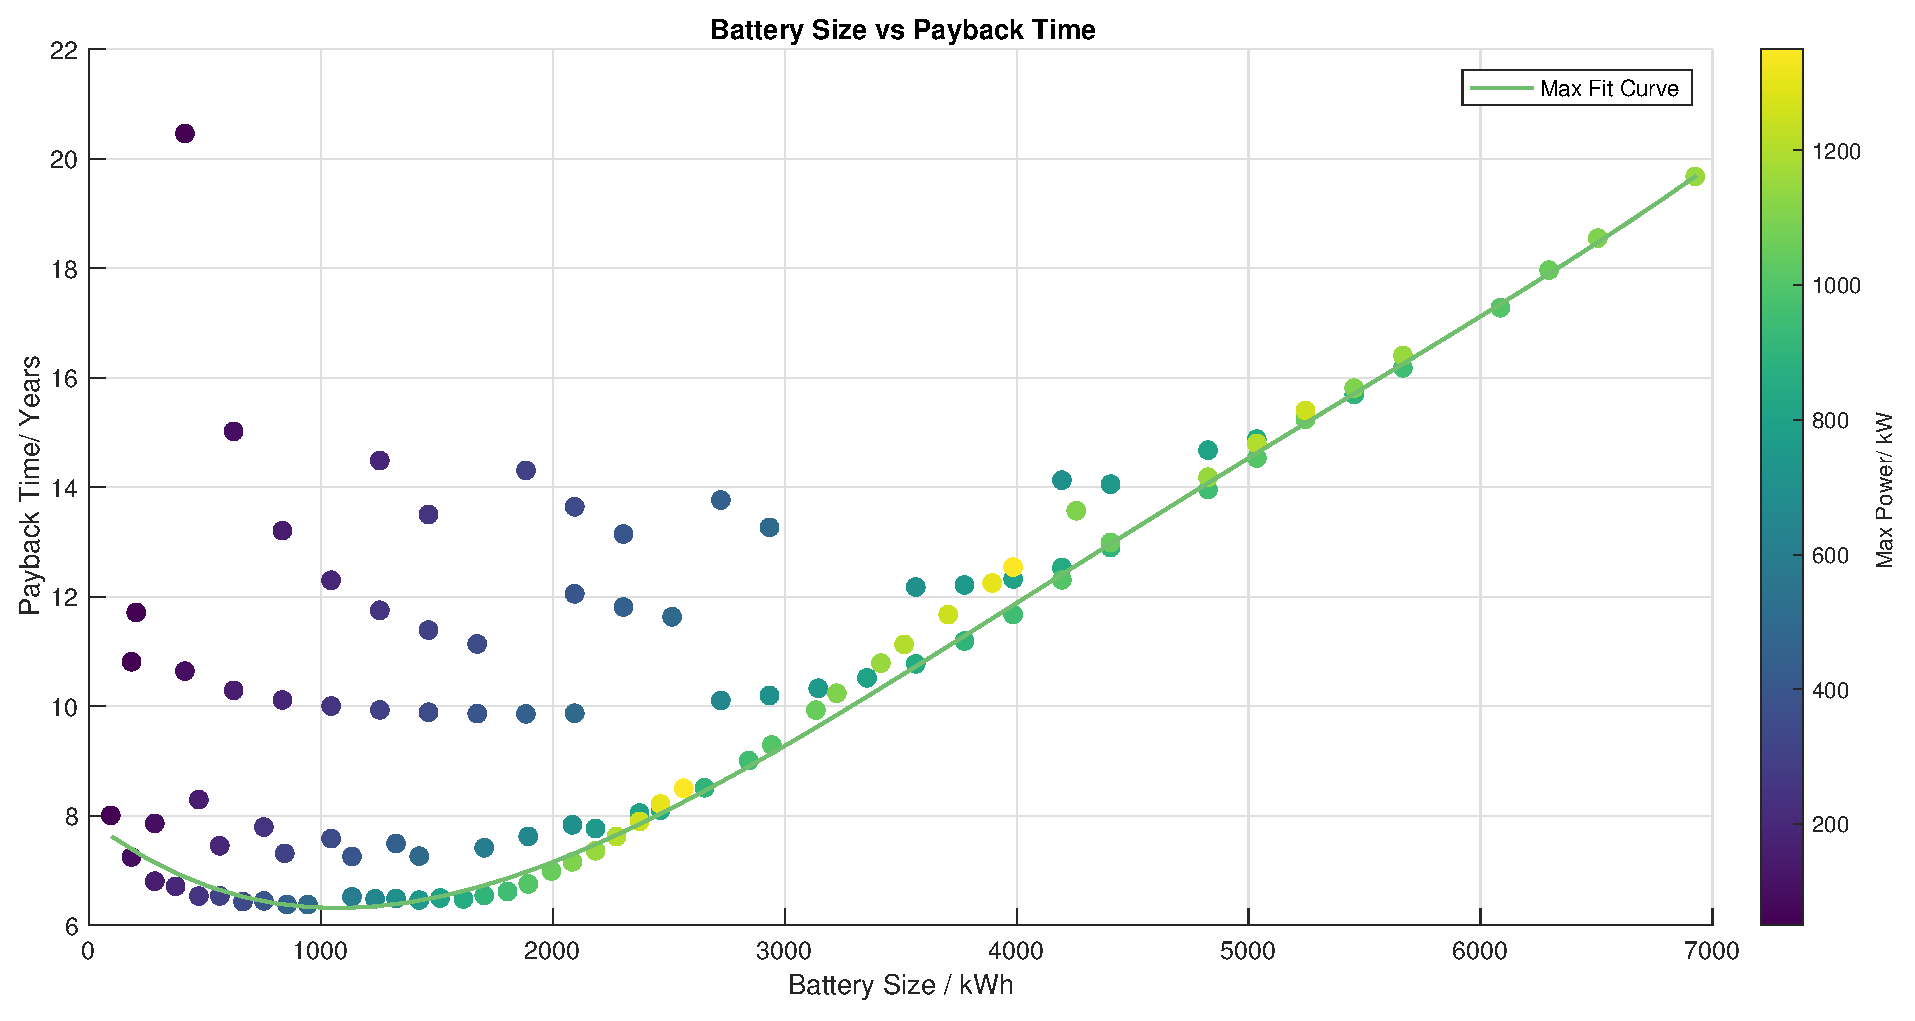
\includegraphics[trim = 0 0 0 0, clip, width=0.7\textwidth]{SRPB2.eps}
 \caption{Graph of Battery Size vs PayBack Time}
 \label{SRPB2}
\end{figure}

Figures \ref{SPA2} and \ref{SRTSPB5} look to use a graphical approach,
of choosing the optimum battery system based on both its capacity and
power rating.

\begin{figure}[H]
\centering
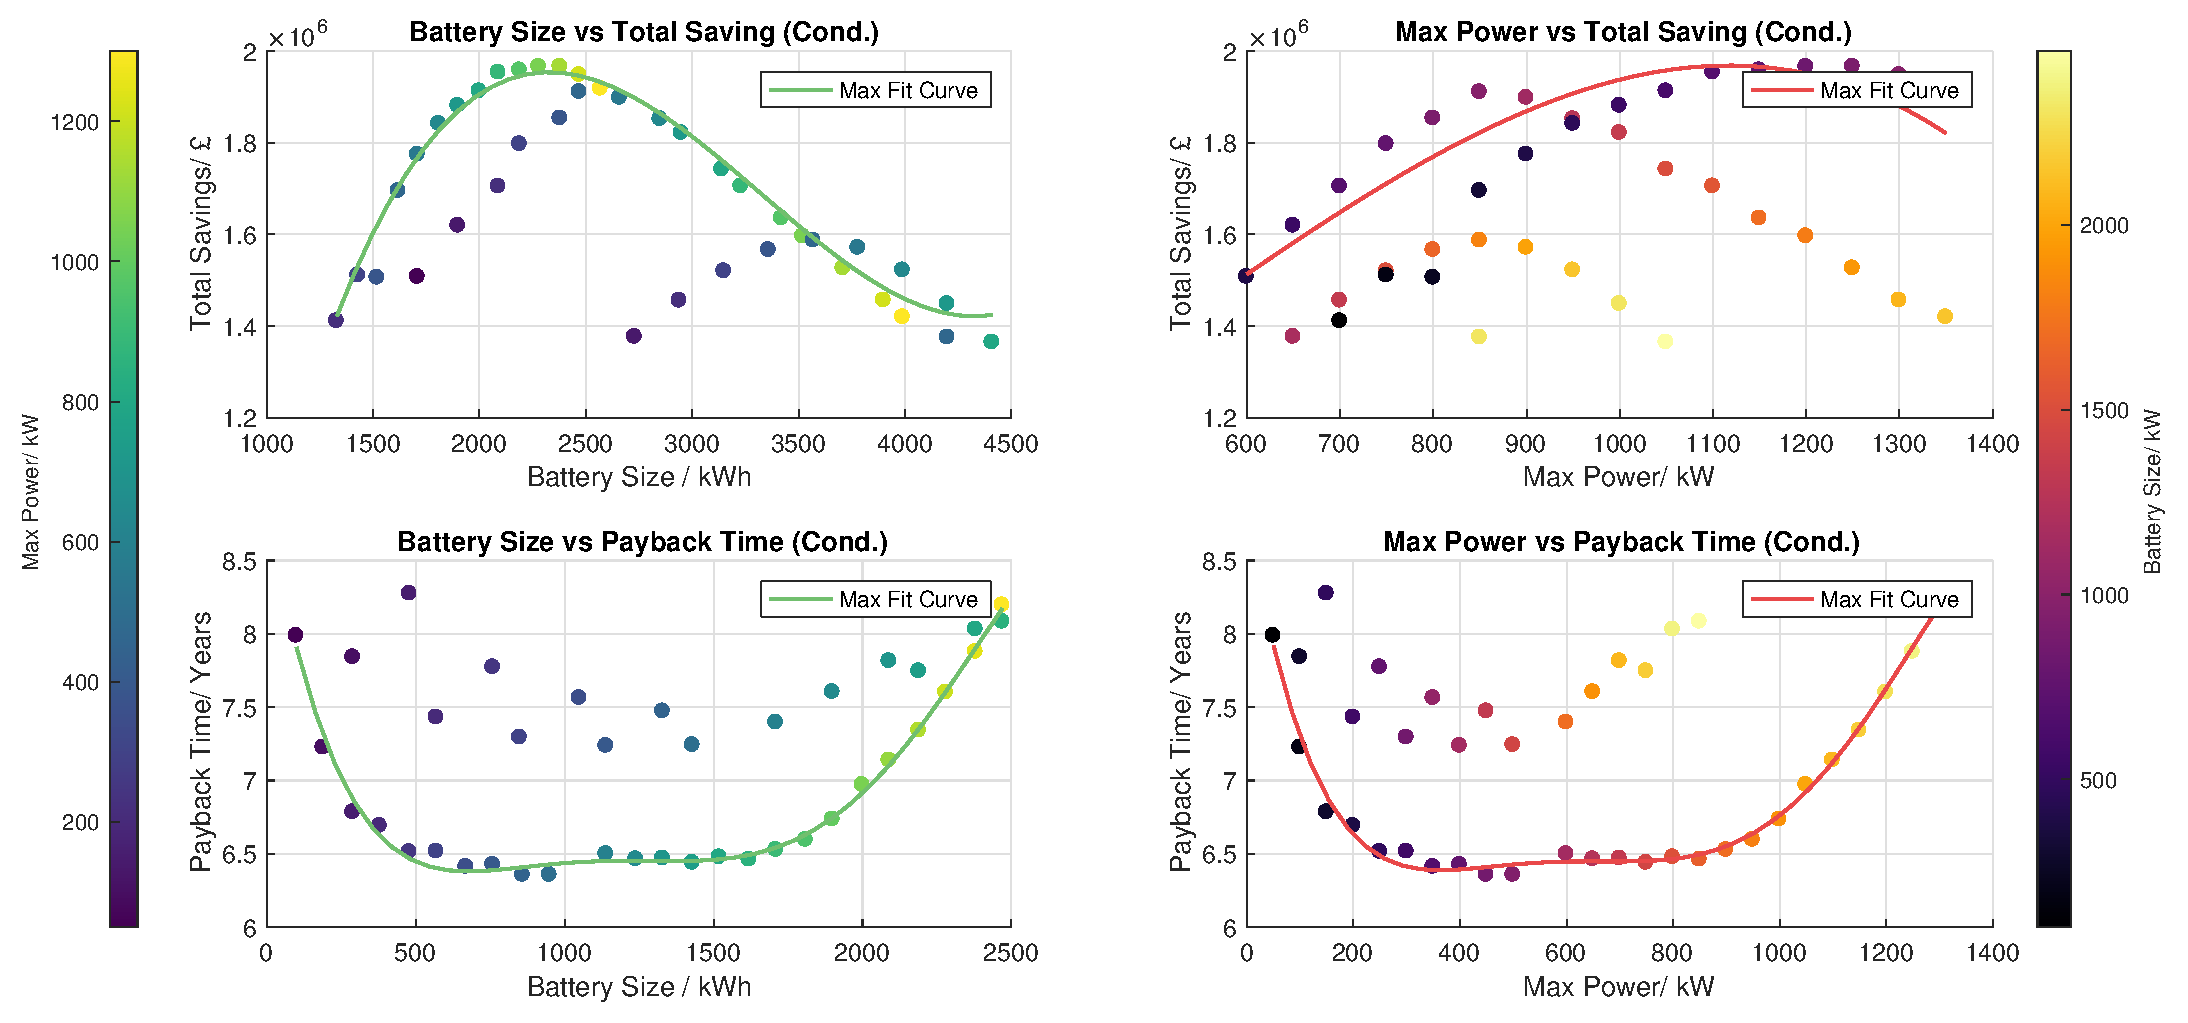
\includegraphics[trim = 0 0 0 0, clip, width=0.9\textwidth]{SPA2.eps}
\caption{Graph Showing Top 30 Batteries with Fitted Curves for both Payback Time and Total Savings}
\label{SPA2}
\end{figure}

A small region either-side of where the two plots cross in Figure
\ref{SPA2}, can be approximated to be the optimum battery battery
parameters. A designer aiming to select a battery based on these two
parameters would look here to make a selection then find the nearest
corresponding battery on the market that fits these values. It is
apparent that the is a very steep drop off in total savings for
batteries that fall outside these bounds. For both max power and total
capacity selecting a battery with a lower rating than this bound will
minimise the payback time, whilst selecting above this region will
increase the payback time exponentially.

\begin{figure}[H]
 \centering
 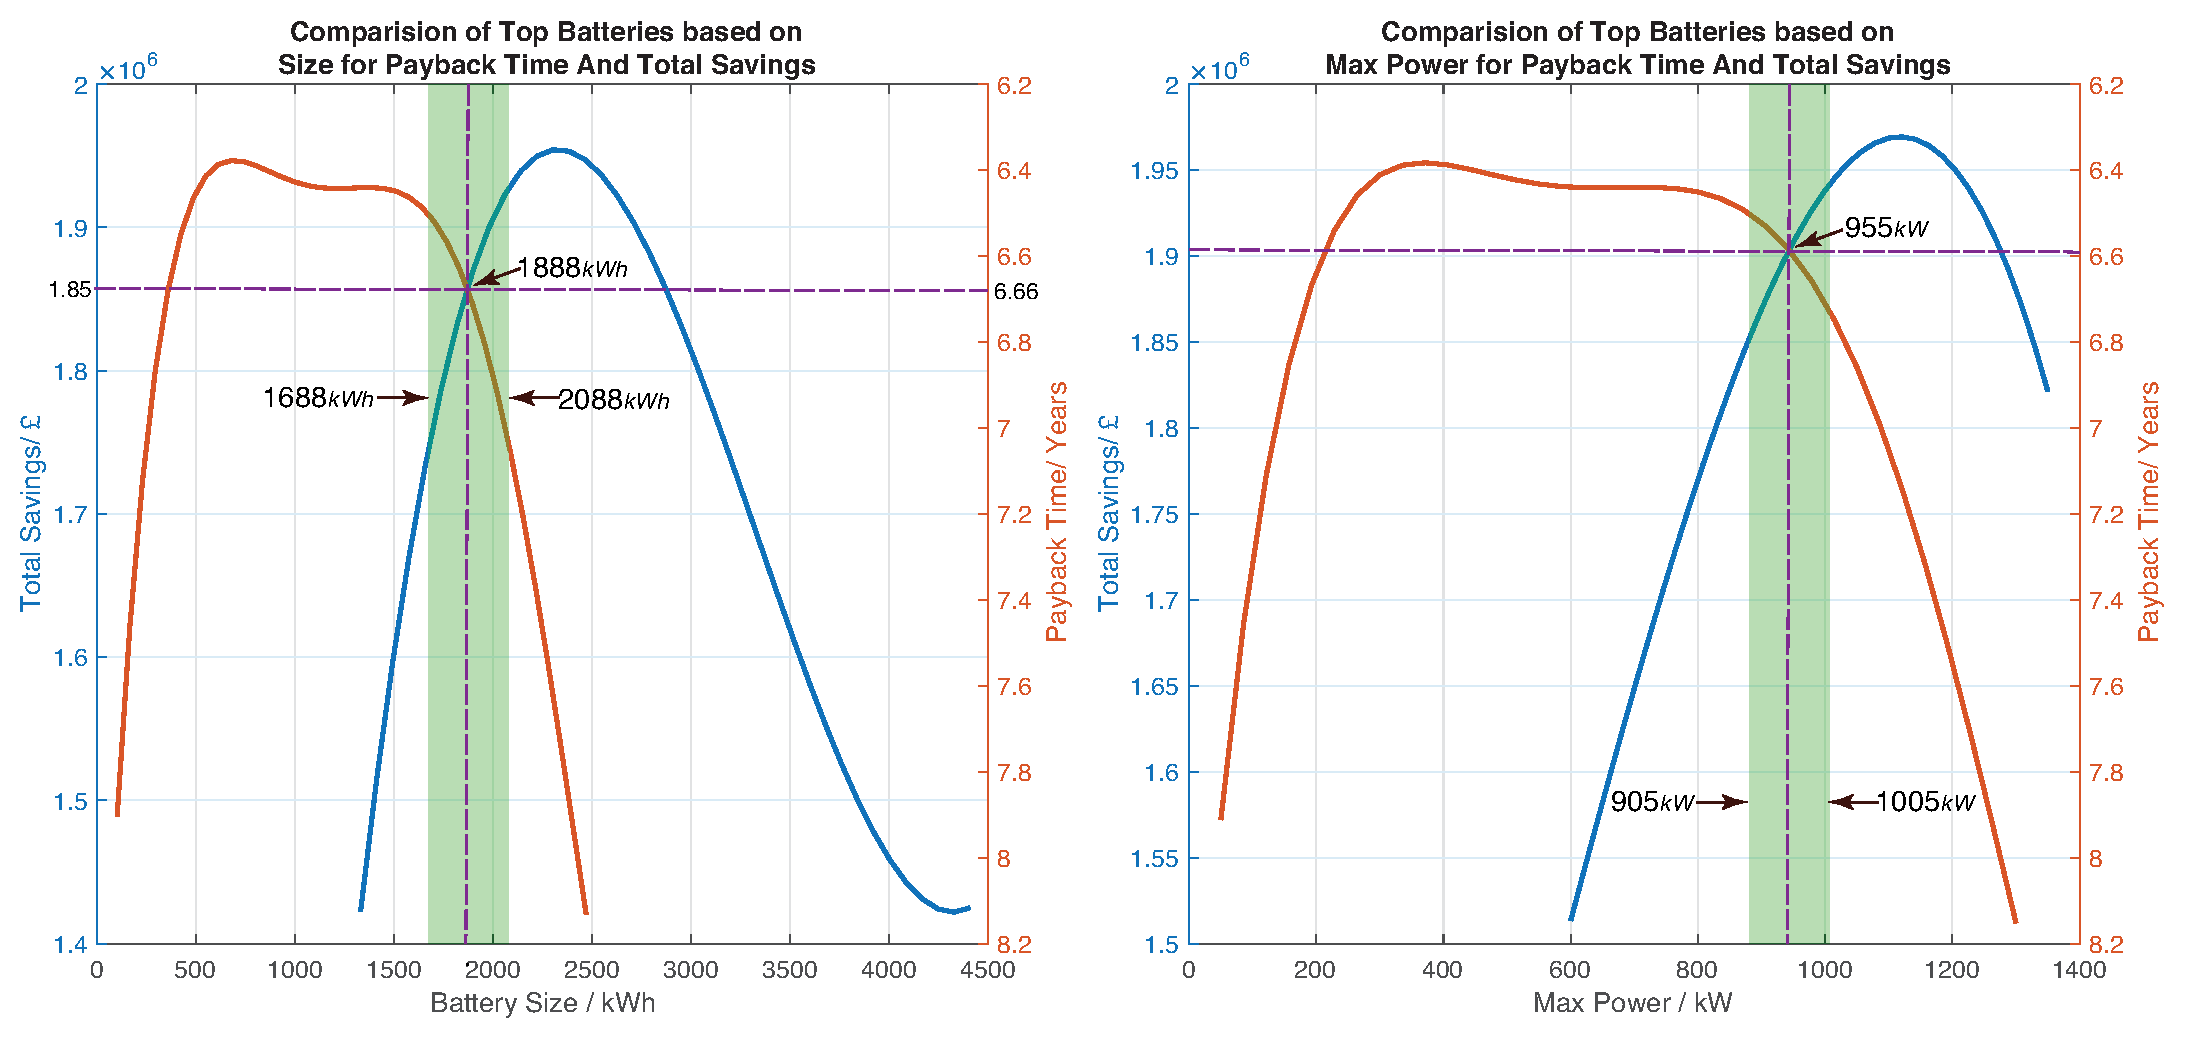
\includegraphics[trim = 0 0 0 0, clip, width=0.9\textwidth]{SRTSPB5ed2.eps}
 \caption{Comparison Between Fit Curves for Payback Period and Total Savings}
 \label{SRTSPB5}
 \end{figure}

Payback period is important measure when evaluating the investments
risk. The longer the pay back period the more time there is for the
battery to fail. For the Tesla Power-pack modelled, the batteries have a
10 year warranty. These reduces the risk significantly if the investment
were to fail before this period. There are other risks associated with
long payback periods are energy pricing changing significantly reducing
the value that the battery creates. Energy contracts typically last no
longer than 4 years,\hl{find reference} in which billing structure could
result in the batteries value dropping to zero -
\hl{add sensitivity analysis}. Knowing that \(\frac{2}{3}\) of the
investment has been paid back as opposed to only a \(\frac{1}{2}\) or
less can have dramatic effects on the risk of the investment. These
factors should be considered when choosing the design region of battery
selection.

\subsubsection{NPV}\label{npv}

An alternate way which tries to quantify risk, is by using net present
value. Three rates of 3\%, 7\% and 12\% were selected to understand the
value of the different batteries. Figure \ref{SRNPV1}, shows the NPV of
the different batteries at these different rates.

\begin{figure}[H]
 \centering
 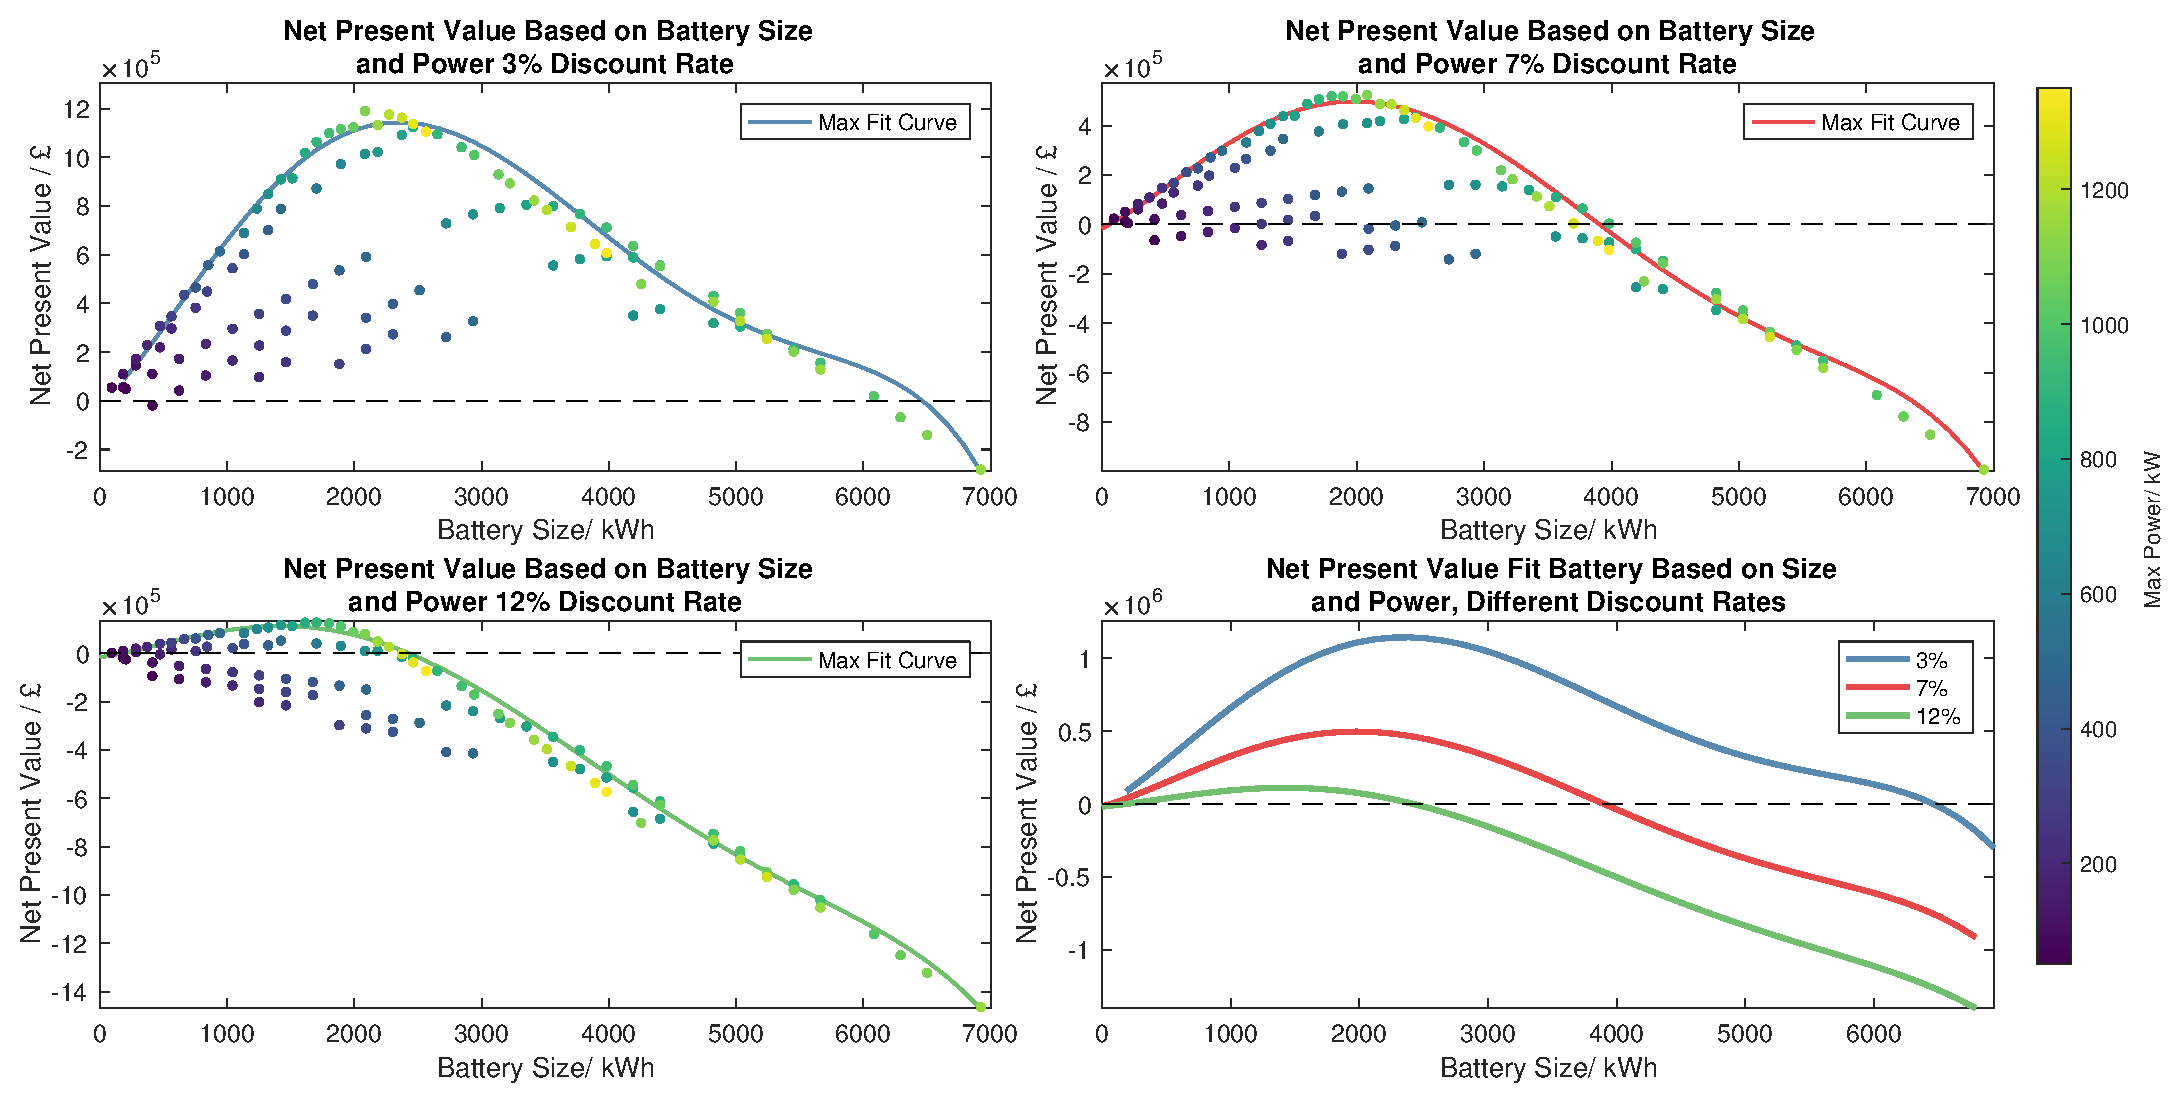
\includegraphics[trim = 0 0 0 0, clip, width=0.9\textwidth]{SRNPV1.eps}
 \caption{Net Present value at Different Discount Rates - Comparison}
 \label{SRNPV1}
\end{figure}

For discount rates of 3\% and 7\% the battery with the highest value was
the same, having a power rating of 1100 kW and a capacity of 2090kWh.
When the discount rate is increased much above 7\%, it can be seen that
the number of batteries that have a positive value is significantly
reduced. The best value battery also becomes smaller rated to only 900kW
and 1710kWh.

Selecting an appropriate discount rate is therefore key for deciding
which is the best investment if using net present value. As the battery
will degrade each year until it reaches its end of life value, it could
be argued that the value of the asset decreases proportionally with this
the remaining life of the battery. Looking at the the optimum battery at
a discount rate of 7\% (see Table \ref{BestNPVTable} below), it can be
seen that the specific battery ran for 4904 cycles. Based on this
assumption the value of the battery would be 98\% of it's original rate,
this works out at a discount rate of roughly 3.92\%. As this will be
different for each batteries the discount rate based on remaining value
alone must approximate all batteries a value of 3\% therefore seems
fair. Discount rate also takes into account inflation. For the UK this
rate has varied between -0.1\% and 3.5\% for the last 5 years
\cite{UnitedKi95:online}.An approximate value of 2\% could be added to
the discount rate to incorporate how money now is worth more than money
later.

Finally discount rates can be used to incorporate interests on loans. As
the battery would be a large one off payment that could be included in
the mortgage on the new campus. This would keep the interest rate low,
which can be approximated to 2\%. Using these three approximations gives
a discount rate of around 7\% shown in figure \ref{SRNPV1}.

\subsubsection{Discussion on Optimum
Battery}\label{discussion-on-optimum-battery}

Below is a table showing the results of the battery which held the best
NPV at a discount rate of 7\%:

\begin{table}[H]
\begin{tabular}{p{3.4cm}p{3cm}p{3cm}}
\textit{Parameter} & \textit{NPV Value} & \textit{Best Value}\\
\textbf{Battery Power Rating}:& 1100 kW\\
\textbf{Battery Capacity}:& 2090 kWh\\
\textbf{Total Saved}:& £1,953,706 & £1,966,697\\
\textbf{Payback Period}:& 7.0959 Years & 6.3562 Years\\
\textbf{Mean DoD}:& 31.5759\% \\
\textbf{Cycles}:& 4904\\
\textbf{Years}:& 25\\
\end{tabular}
\label{BestNPVTable}
\caption{Table Showing the Best Battery Results based on a Net Present Value of 7\%}
\end{table}

Comparing the results between Net Present Value and the Total Saving Vs
Payback plots (see Figure \ref{SRTSPB5}),shows that the recommendation
of NPV at 7\% is larger than the recommendation from the total saving
payback plot. This suggests that at this discount rate, total savings is
worth more than a reduced payback time.

\subsubsection{Battery Usage and Secondary
Analysis}\label{battery-usage-and-secondary-analysis}

\begin{figure}[H]
 \centering
 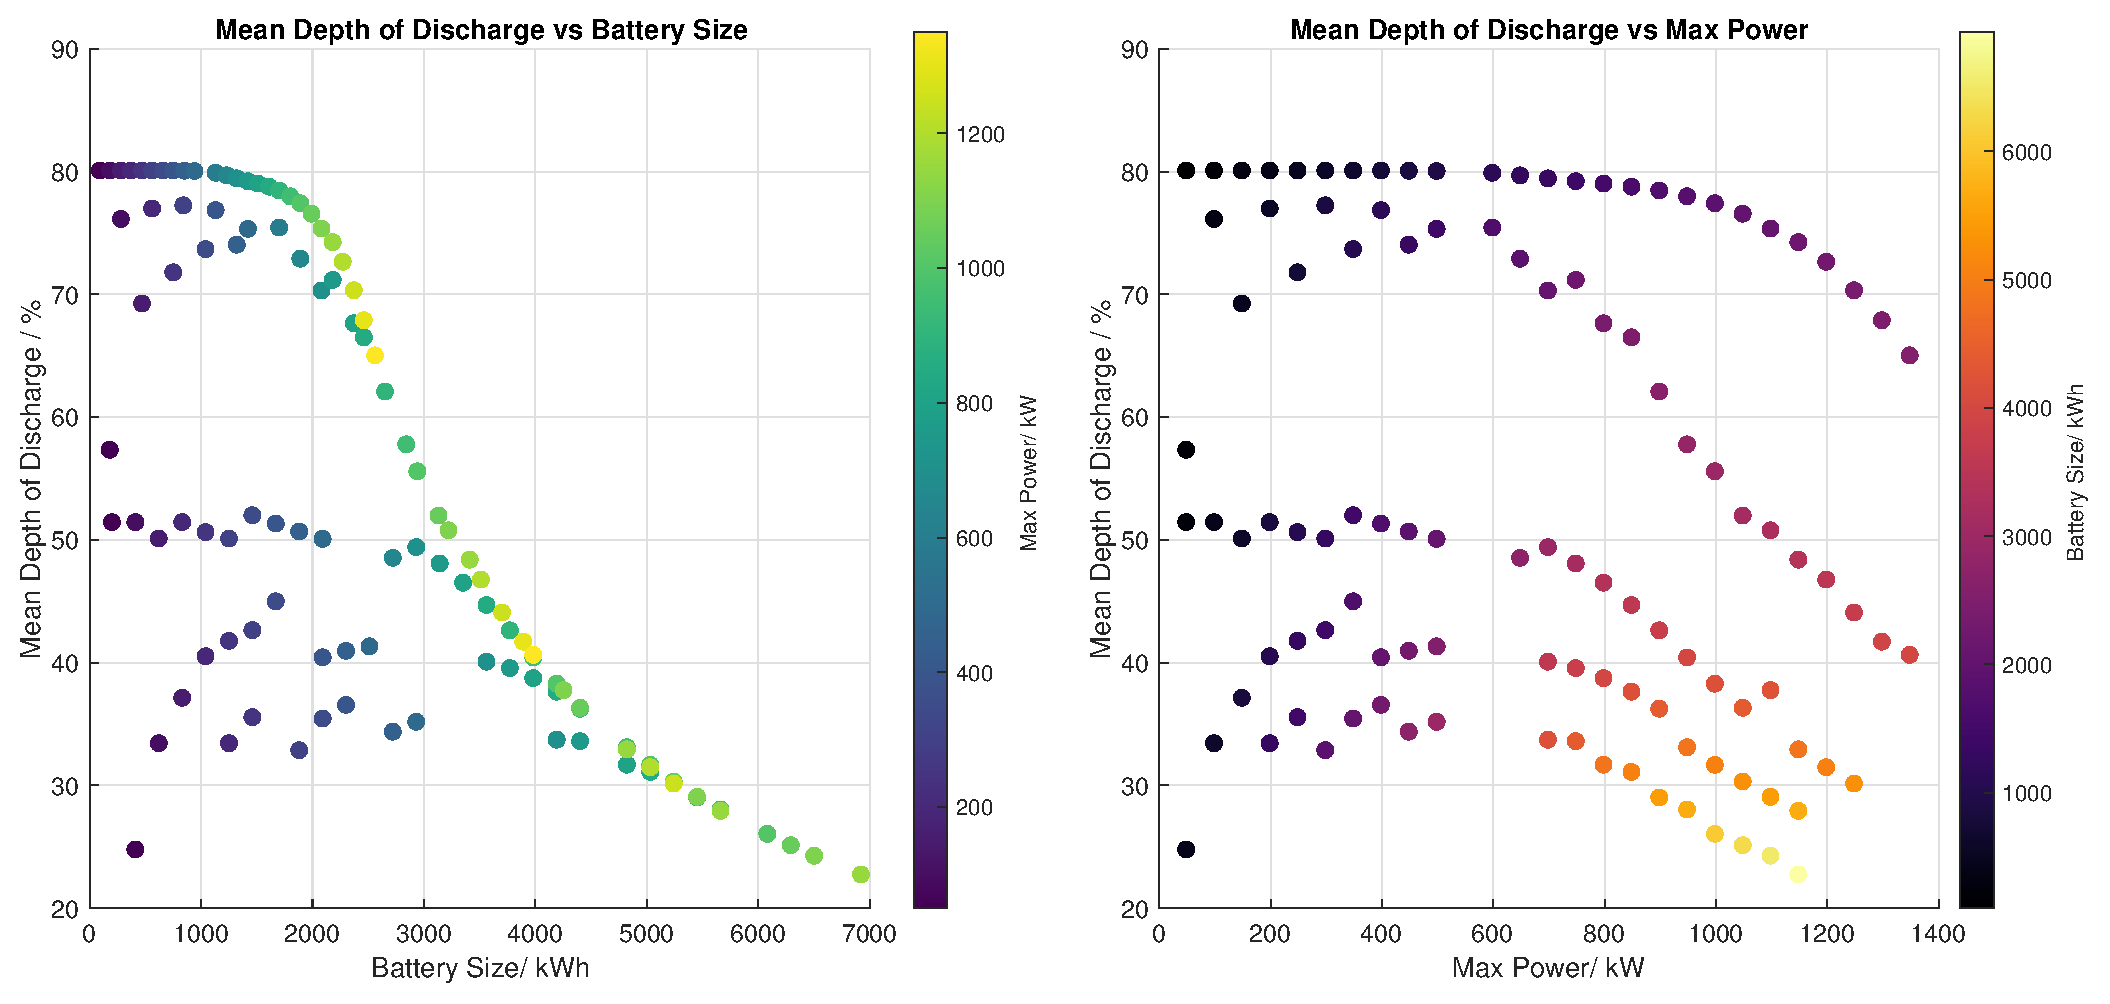
\includegraphics[trim = 0 0 0 0, clip, width=0.7\textwidth]{DOD1.eps}
\caption{Depth of Discharge For Battery Lifetime}
 \label{DOD1}
 \end{figure}

\begin{itemize}
\tightlist
\item
  Battery depth of discharge can vary greatly depending on the power
  rating and capacity, a trend can be seen as two separate
\end{itemize}

\section{Conclusions and Future Work}\label{conclusions-and-future-work}

\subsection{Conclusions}\label{conclusions}

\subsection{Future Work}\label{future-work}

\newpage

\section{Appendices}

\begin{figure}[H]
\centering
\includegraphics[width=1\textwidth]{battypes}
\caption{Diagram Showing Batteries Catorgised for Their Use Case \cite{Dunn928}}
\label{battypes}
\end{figure}

\begin{landscape}

\begin{table}[H]
\centering
\includegraphics[width=1.3\textwidth]{battab.eps}
\caption{Table Showing Battery Performance}
\label{battabs}
\end{table}

\end{landscape}
% -----------------------------------------------------------------------------------
%                                  APENDIX
% -----------------------------------------------------------------------------------
\end{counted} %<<<<<<<<<<<<<<ENDS WORD COUNTER
Above were \thewords\ words. %<<<<<<<<<<<<<<DISPLAYS WORD COUNTER
% -----------------------------------------------------------------------------------
%                               BIBLIOGRAPHY - Insert Name of BIB File Here
% -----------------------------------------------------------------------------------
\newpage

% ---------------BIBTEX OLD-----------------------------------------------------
% \bibliographystyle{unsrt} %%%% Plain or alpha can change orders here
% \bibliography{BibFile}
% \nocite{*} %%%if you want to see all references even those note cited in the text
% -----------------------------------------------------------------------------------

\printbibliography

\end{document}
